%%%%%%%%%%%%%%%%%%%%%%%%%%%%%%%%%%%%%%%%%%%%%%%%%%
\section{Additional Experiments}
\label{app:sec:additional_experiments}
%%%%%%%%%%%%%%%%%%%%%%%%%%%%%%%%%%%%%%%%%%%%%%%%%%
\subsection{1D Regression}
\label{app:sec:additional_experiments:1dregression}

\begin{table}[t]
\centering
\setlength{\tabcolsep}{0.3em}
\caption{Test results for 1D regression tasks on RBF, Matern, Periodic, and $t$-noise. `Context' and `Target' respectively denote context and target log-likelihood values, and `Task' denotes the task log-likelihood. All values are averaged over four seeds.}
\label{table/app_gp_inf_full}
\resizebox{\linewidth}{!}{
\begin{tabular}{lrrrrrrrrrrrr}
\toprule
      & \multicolumn{3}{c}{RBF} & \multicolumn{3}{c}{Matern} & \multicolumn{3}{c}{Periodic} & \multicolumn{3}{c}{$t$-noise} \\
\cmidrule(lr){2-4}\cmidrule(lr){5-7}\cmidrule(lr){8-10}\cmidrule(lr){11-13}
Model & Context & Target & Task & Context & Target & Task & Context & Target & Task & Context & Target & Task \\
\midrule
CNP & 
 1.096$\spm{0.023}$ &  0.515$\spm{0.018}$ &  0.796$\spm{0.020}$ &
 1.031$\spm{0.010}$ &  0.347$\spm{0.006}$ &  0.693$\spm{0.008}$ &
-0.120$\spm{0.020}$ & -0.729$\spm{0.004}$ & -0.363$\spm{0.012}$ &
 0.032$\spm{0.014}$ & -0.816$\spm{0.032}$ & -0.260$\spm{0.012}$ \\
NP & 
 1.022$\spm{0.005}$ &  0.498$\spm{0.003}$ &  0.748$\spm{0.004}$ &
 0.948$\spm{0.006}$ &  0.337$\spm{0.005}$ &  0.641$\spm{0.005}$ &
-0.267$\spm{0.024}$ & \textBF{-0.668}$\spm{0.006}$ & -0.441$\spm{0.013}$ &
 \textBF{0.201}$\spm{0.025}$ & -0.333$\spm{0.078}$ & \textBF{-0.038}$\spm{0.026}$ \\
BNP & 
 1.112$\spm{0.003}$ &  0.588$\spm{0.004}$ &  0.841$\spm{0.003}$ &
 1.057$\spm{0.009}$ &  0.418$\spm{0.006}$ &  0.741$\spm{0.007}$ &
-0.106$\spm{0.017}$ & -0.705$\spm{0.001}$ & -0.347$\spm{0.010}$ &
-0.009$\spm{0.032}$ & -0.619$\spm{0.191}$ & -0.217$\spm{0.036}$ \\
\textBF{MPNP (ours)} & 
 \textBF{1.189}$\spm{0.005}$ &  \textBF{0.675}$\spm{0.003}$ &  \textBF{0.911}$\spm{0.003}$ &
 \textBF{1.123}$\spm{0.005}$ &  \textBF{0.481}$\spm{0.007}$ &  \textBF{0.796}$\spm{0.005}$ &
 \textBF{0.205}$\spm{0.020}$ & \textBF{-0.668}$\spm{0.008}$ & \textBF{-0.171}$\spm{0.013}$ &
 0.145$\spm{0.017}$ & \textBF{-0.329}$\spm{0.025}$ & -0.061$\spm{0.012}$ \\
\midrule
CANP & 
 1.304$\spm{0.027}$ &  0.847$\spm{0.005}$ &  1.036$\spm{0.020}$ &
 1.264$\spm{0.041}$ &  0.662$\spm{0.013}$ &  0.937$\spm{0.031}$ &
 0.527$\spm{0.106}$ & -0.592$\spm{0.002}$ &  0.010$\spm{0.069}$ &
 0.410$\spm{0.155}$ & -0.577$\spm{0.022}$ & -0.008$\spm{0.098}$ \\
ANP & 
 \textBF{1.380}$\spm{0.000}$ &  0.850$\spm{0.007}$ &  1.090$\spm{0.003}$ &
 \textBF{1.380}$\spm{0.000}$ &  0.663$\spm{0.004}$ &  1.019$\spm{0.002}$ &
 0.583$\spm{0.011}$ & -1.019$\spm{0.023}$ &  0.090$\spm{0.004}$ &
 0.836$\spm{0.071}$ & -0.415$\spm{0.131}$ &  0.374$\spm{0.034}$ \\
BANP & 
 \textBF{1.380}$\spm{0.000}$ &  0.846$\spm{0.001}$ &  1.088$\spm{0.000}$ &
 \textBF{1.380}$\spm{0.000}$ &  0.662$\spm{0.005}$ &  1.018$\spm{0.002}$ &
 \textBF{1.354}$\spm{0.006}$ & -0.496$\spm{0.005}$ &  \textBF{0.634}$\spm{0.005}$ &
 0.646$\spm{0.042}$ & -0.425$\spm{0.050}$ &  0.270$\spm{0.033}$ \\
\textBF{MPANP (ours)} & 
 1.379$\spm{0.000}$ &  \textBF{0.881}$\spm{0.003}$ &  \textBF{1.102}$\spm{0.001}$ &
 \textBF{1.380}$\spm{0.000}$ &  \textBF{0.692}$\spm{0.003}$ &  \textBF{1.029}$\spm{0.001}$ &
 1.348$\spm{0.005}$ & \textBF{-0.494}$\spm{0.007}$ &  0.630$\spm{0.005}$ &
 \textBF{0.842}$\spm{0.062}$ & \textBF{-0.332}$\spm{0.026}$ &  \textBF{0.384}$\spm{0.041}$ \\
\bottomrule
\end{tabular}}
\end{table}

\paragraph{Full results for~\cref{table/main_gp_inf}}
We provide the full test results for 1D regression tasks including context, target, and task log-likelihood values in~\cref{table/app_gp_inf_full}.

\paragraph{Increasing the encoder size of baselines}
\begin{table}[t]
\centering
\caption{Further comparisons with baselines with increased number of parameters. `Context' and `Target' respectively denote context and target log-liklihood values, and `Task' denotes the task log-likelihood. All values are averaged over four seeds.}
\label{table/app_gp_inf_sizeup}
\resizebox{\linewidth}{!}{
\begin{tabular}{lrrrrrrr}
\toprule
      & & \multicolumn{3}{c}{RBF} & \multicolumn{3}{c}{Matern} \\
\cmidrule(lr){3-5}\cmidrule(lr){6-8}
Model & \# Params & Context & Target & Task & Context & Target & Task \\
\midrule
CNP & 264 K & 
1.096$\spm{0.008}$ & 0.517$\spm{0.007}$ & 0.797$\spm{0.007}$ &
1.017$\spm{0.021}$ & 0.340$\spm{0.012}$ & 0.681$\spm{0.017}$ \\
NP  & 274 K & 
1.026$\spm{0.004}$ & 0.501$\spm{0.003}$ & 0.752$\spm{0.003}$ &
0.948$\spm{0.005}$ & 0.334$\spm{0.002}$ & 0.640$\spm{0.003}$ \\
BNP & 261 K & 
1.115$\spm{0.007}$ & 0.591$\spm{0.005}$ & 0.843$\spm{0.006}$ &
1.051$\spm{0.007}$ & 0.416$\spm{0.005}$ & 0.736$\spm{0.005}$ \\
\textBF{MPNP (ours)} & 266 K &
\textBF{1.189}$\spm{0.005}$ & \textBF{0.675}$\spm{0.003}$ & \textBF{0.911}$\spm{0.003}$ &
\textBF{1.123}$\spm{0.005}$ & \textBF{0.481}$\spm{0.007}$ & \textBF{0.796}$\spm{0.005}$ \\
\midrule
CANP & 868 K & 
1.305$\spm{0.007}$ & 0.844$\spm{0.006}$ & 1.035$\spm{0.005}$ &
1.278$\spm{0.013}$ & 0.663$\spm{0.006}$ & 0.947$\spm{0.008}$ \\
ANP  & 877 K & 
\textBF{1.380}$\spm{0.000}$ & 0.858$\spm{0.002}$ & 1.093$\spm{0.001}$ &
\textBF{1.380}$\spm{0.000}$ & 0.668$\spm{0.006}$ & 1.020$\spm{0.002}$ \\
BANP & 885 K & 
1.379$\spm{0.001}$ & 0.839$\spm{0.015}$ & 1.085$\spm{0.007}$ &
1.376$\spm{0.005}$ & 0.652$\spm{0.032}$ & 1.012$\spm{0.014}$ \\
\textBF{MPANP (ours)} & 877 K &
1.379$\spm{0.000}$ & \textBF{0.881}$\spm{0.003}$ & \textBF{1.102}$\spm{0.001}$ &
\textBF{1.380}$\spm{0.000}$ &  \textBF{0.692}$\spm{0.003}$ &  \textBF{1.029}$\spm{0.001}$ \\
\bottomrule
\end{tabular}}
\end{table}

Since the generator increases the size of the encoder in \glspl{mpnp}, one can claim that the performance gain of \glspl{mpnp} may come from the increased model size. To verify this, we increased the hidden dimensions of the encoder of baselines and compared them with ours. The results displayed in~\cref{table/app_gp_inf_sizeup} further clarify that ours still outperforms the baselines even when the number of parameters gets in line.


\subsection{High-D Regression}
% \paragraph{Settings}
We conducted additional experiments on the synthetic high-dimensional regression data (i.e., generating one-dimensional y from four-dimensional x with RBF kernel). Here we used the same model structures with the 1D regression task except for the input layer, and the same settings for the RBF kernel with 1D regression except for $l\sim \text{Unif}(0.5, 3.0)$. We fixed the base learning rate to $0.00015$ for all models throughout the high-dimensional regression experiments.


% \paragraph{Results}
\cref{table/app_high_d} clearly shows our \glspl{mpnp} still outperform baselines for log-likelihood values we measured.


\begin{table}[t]
\centering

\caption{Test results for 4D regression tasks on RBF. `Context' and `Target' respectively denote context and target log-likelihood values, and `Task' denotes the task log-likelihood. All values are averaged over four seeds.}
\label{table/app_high_d}

\begin{tabular}{lrrr}
\toprule
& \multicolumn{3}{c}{RBF}  \\
\cmidrule(lr){2-4}
Model & Context & Target & Task  \\
\midrule
CNP & 0.572$\spm{0.003}$ &  0.265$\spm{0.002}$ &  0.410$\spm{0.003}$ \\
NP  & 0.568$\spm{0.009}$ &  0.267$\spm{0.004}$ &  0.407$\spm{0.007}$ \\
BNP & 0.621$\spm{0.015}$ &  0.323$\spm{0.008}$ &  0.467$\spm{0.013}$ \\
\textBF{MPNP (ours)} & 
\textBF{0.820}$\spm{0.002}$ & \textBF{0.441}$\spm{0.004}$ & \textBF{0.633}$\spm{0.004}$ \\
\midrule
CANP & 0.957$\spm{0.005}$ &  0.585$\spm{0.006}$ &  0.743$\spm{0.005}$  \\
ANP & 1.357$\spm{0.006}$ &  0.320$\spm{0.014}$ &  0.890$\spm{0.007}$  \\
BANP & \textBF{1.380}$\spm{0.000}$ &  0.549$\spm{0.006}$ &  1.013$\spm{0.002}$  \\
\textBF{MPANP (ours)} & 1.379$\spm{0.000}$ &  \textBF{0.645}$\spm{0.007}$ &  \textBF{1.046}$\spm{0.002}$ \\
\bottomrule
\end{tabular}
\end{table}


%%%%%%%%%%%%%%%%%%%%%%%%%%%%%%%%%%%%%%%%%%%%%%%%%%
\subsection{Image Completion}
\label{app:sec:additional_experiments:imagecompletion}

\begin{figure}[t]
    \centering
    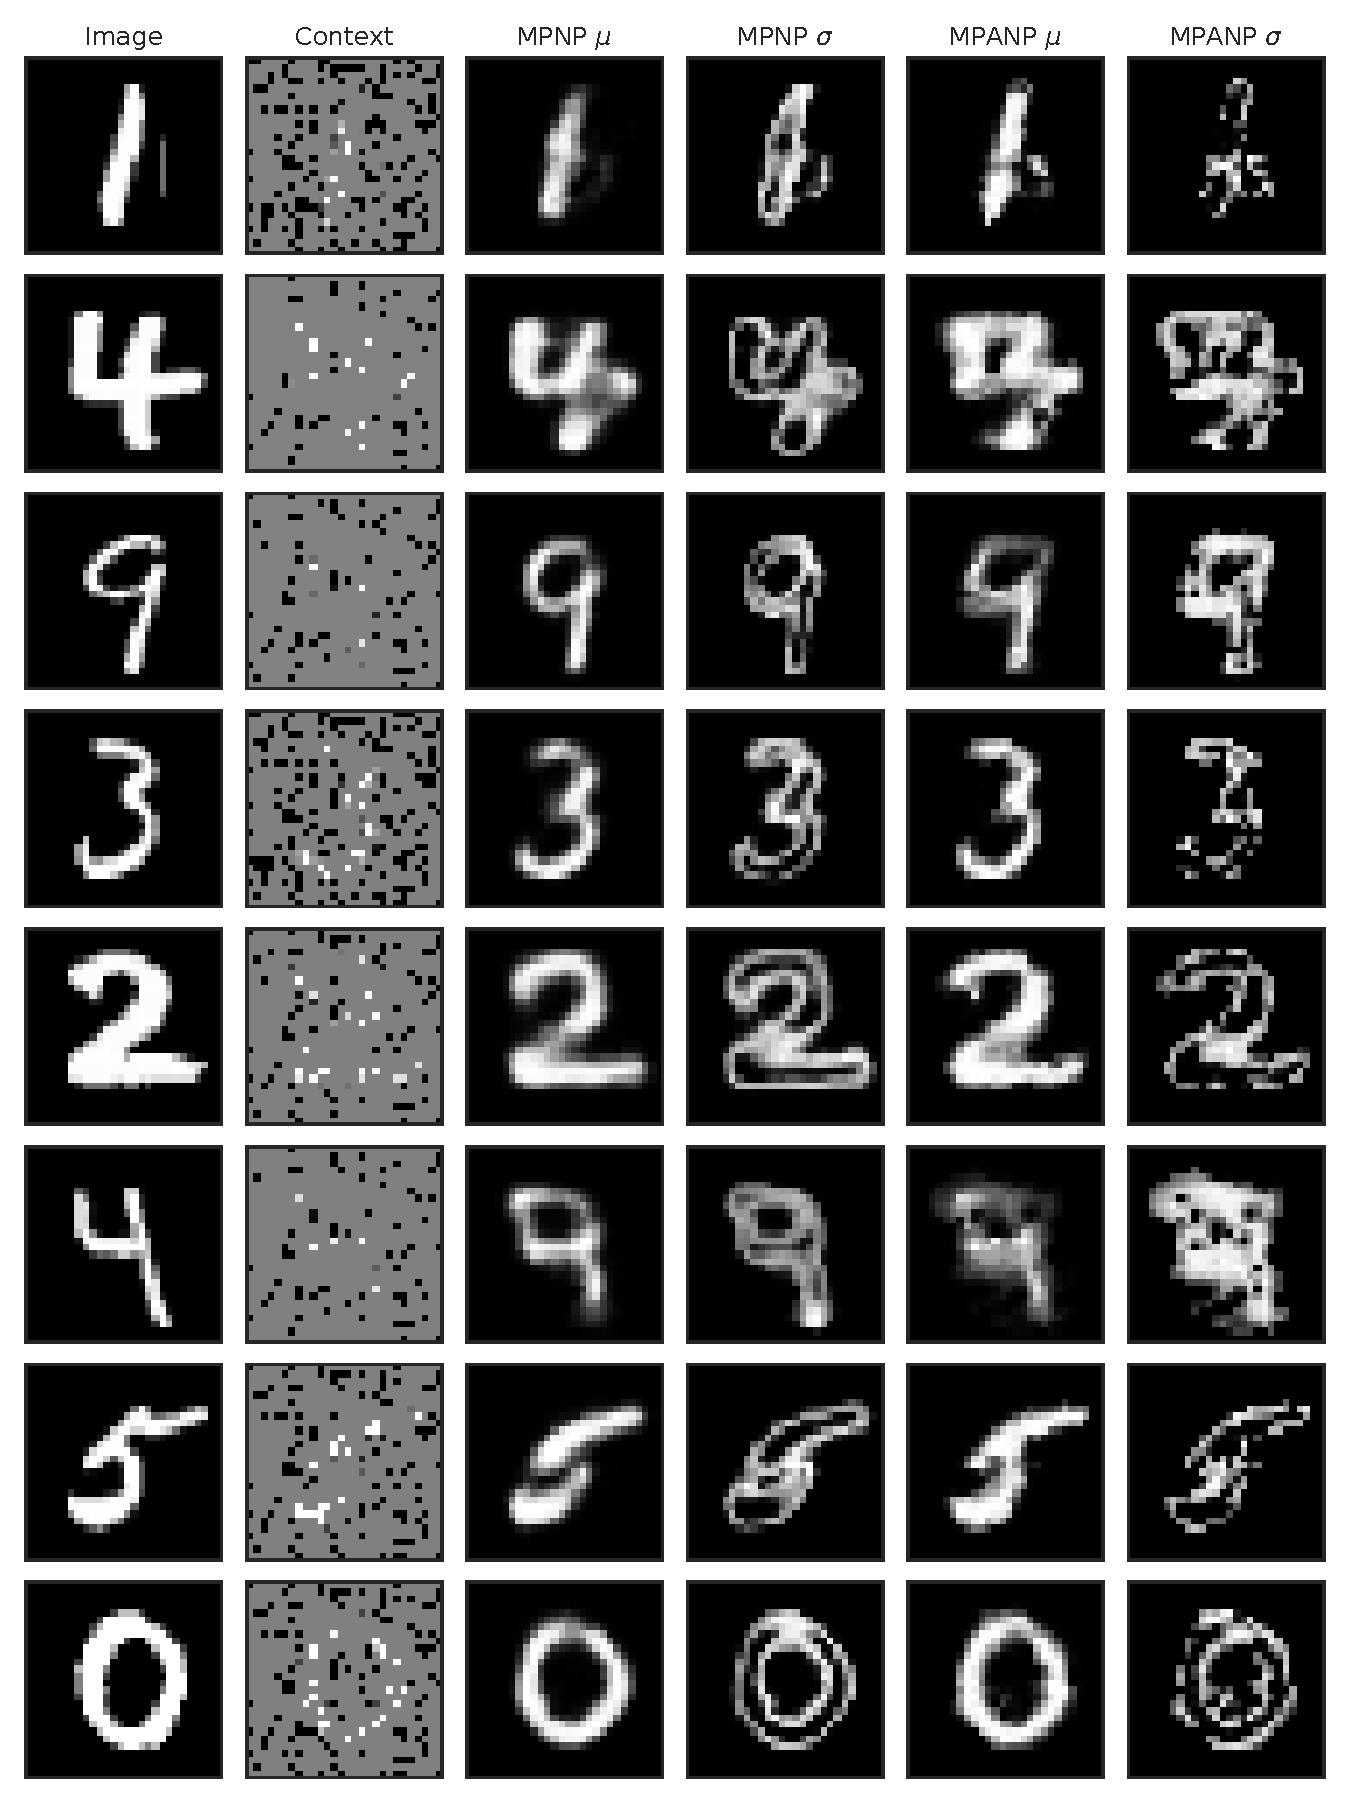
\includegraphics[width = \textwidth]{figure/app_visualize_mnist.pdf}
    \caption{Predicted mean and standard deviation of image pixels by trained \glspl{mpnp} with MNIST dataset. The first column shows the real image from test dataset. The second column shows the context dataset which given to the models. The third and the forth columns show the predicted mean and standard deviation from the \gls{mpnp} respectively. The fifth and the sixth columns show the predicted mean and standard deviation from the \gls{mpanp}.} 
    \label{figure/app_visualize_mnist}
\end{figure}

\begin{figure}
    \centering
    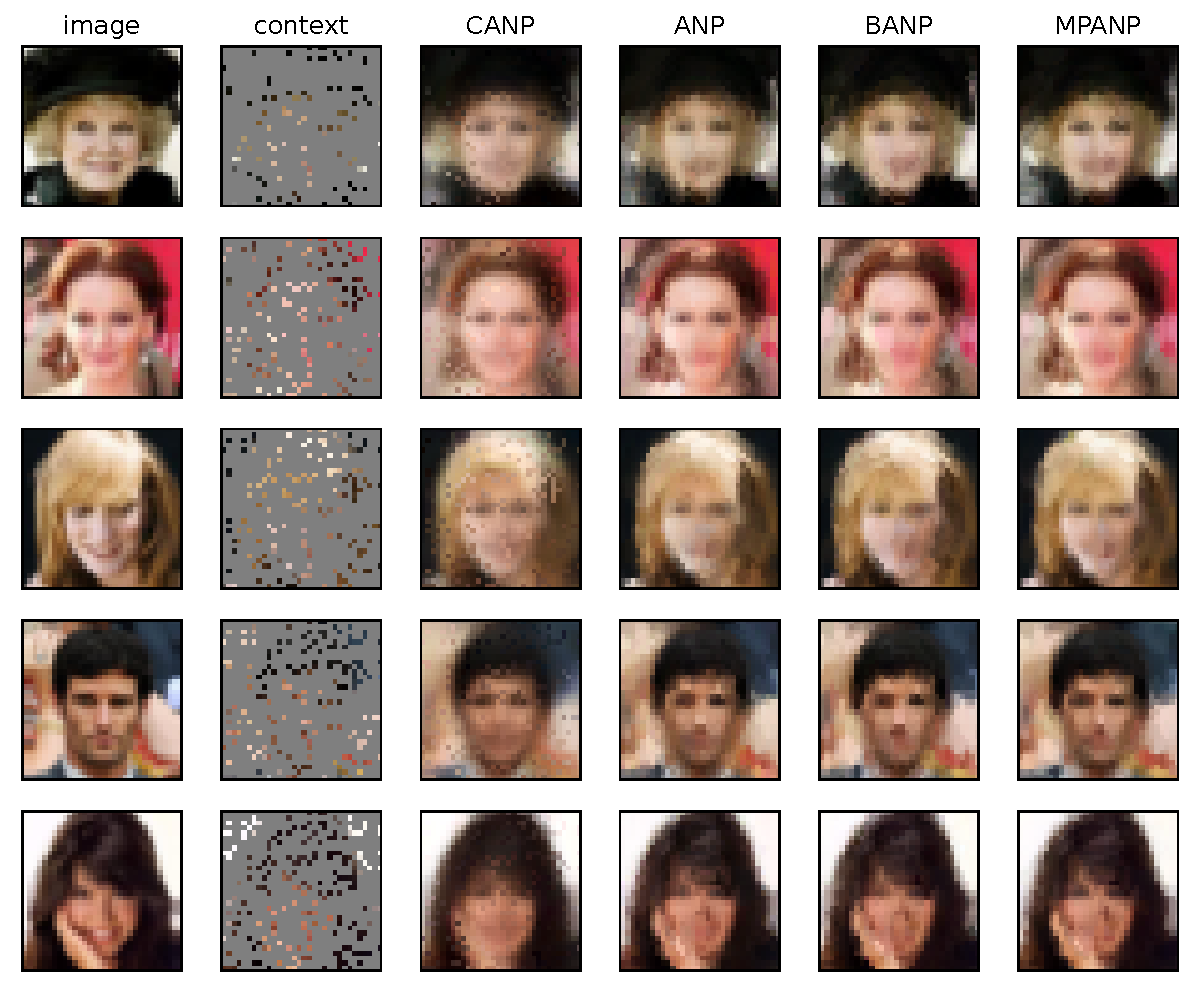
\includegraphics[width=\linewidth]{figure/app_visualize_celeba.pdf}
    \caption{Predicted mean of image pixels by trained \gls{canp}, \gls{anp}, \gls{banp} and \gls{mpanp} model. (Column 1) Here we can see the 5 ground truth real image from the test dataset. (Column 2) The context set which given to the models. (Column 3-6) The predicted mean of image pixels by each models.}
    \label{figure/app_visualize_celeba}
\end{figure}


\paragraph{MNIST}
We provide some completed MNIST images in~\cref{figure/app_visualize_mnist}. It shows that both \gls{mpnp} and \gls{mpanp} successfully fill up the remaining parts of the image for a given context and capture the uncertainties as predictive variances.

\paragraph{CelebA}
We also present five examples from the CelebA dataset in~\cref{figure/app_visualize_celeba}. It shows that \gls{mpanp} provides perceptually reasonable predictions even for complex three-channel images.

% In this section, we presents some examples of the visualizations of completed images along with the uncertainties in terms of predictive variances.
% We report 8 samples for the MNIST dataset.
% In \cref{figure/app_visualize_mnist}, we report the results for the image completion with MNIST test dataset.
% Here we can see that both the \gls{mpnp} and the \gls{mpanp} well complete the remain parts of the image and well capture the uncertainties in terms of predictive variances.

%%%%%%%%%%%%%%%%%%%%%%%%%%%%%%%%%%%%%%%%%%%%%%%%%%
\subsection{Bayesian Optimization}
\label{app:sec:additional_experiments:bo}


\begin{figure}
\centering
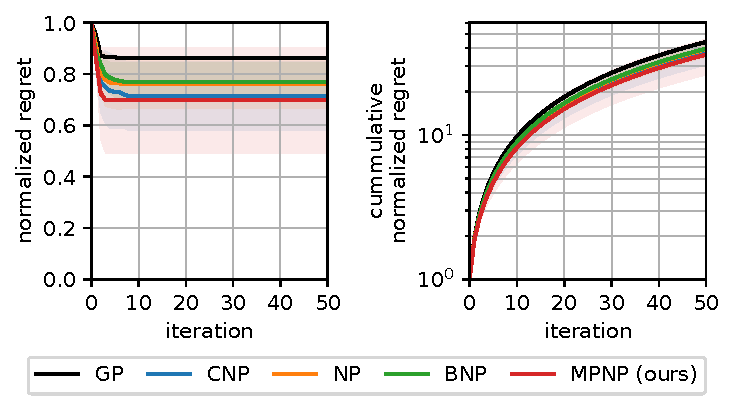
\includegraphics[width=0.49\linewidth]{figure/app_bo_sob_np.pdf}
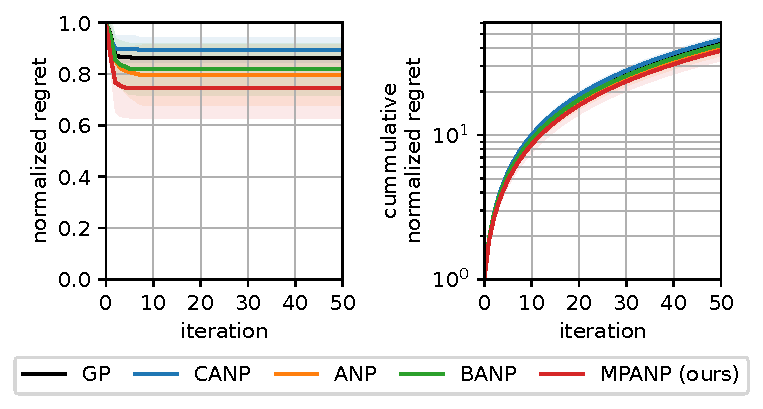
\includegraphics[width=0.49\linewidth]{figure/app_bo_sob_anp.pdf}
\caption{Results for Bayesian optimization on~\citet{sobester2008engineering} function.}
\label{figure/app_bo_sob}
\end{figure}
We provide the results for Bayesian optimization on the~\citet{sobester2008engineering} function in~\cref{figure/app_bo_sob}. Our \glspl{mpnp} consistently outperform baselines as discussed in~\cref{main:sec:experiments:bo}. We also present the visual results for Bayesian optimization in~\cref{figure/app_visualize_bo_np,figure/app_visualize_bo_anp}.

\begin{figure}
\centering
\begin{subfigure}[b]{\textwidth}
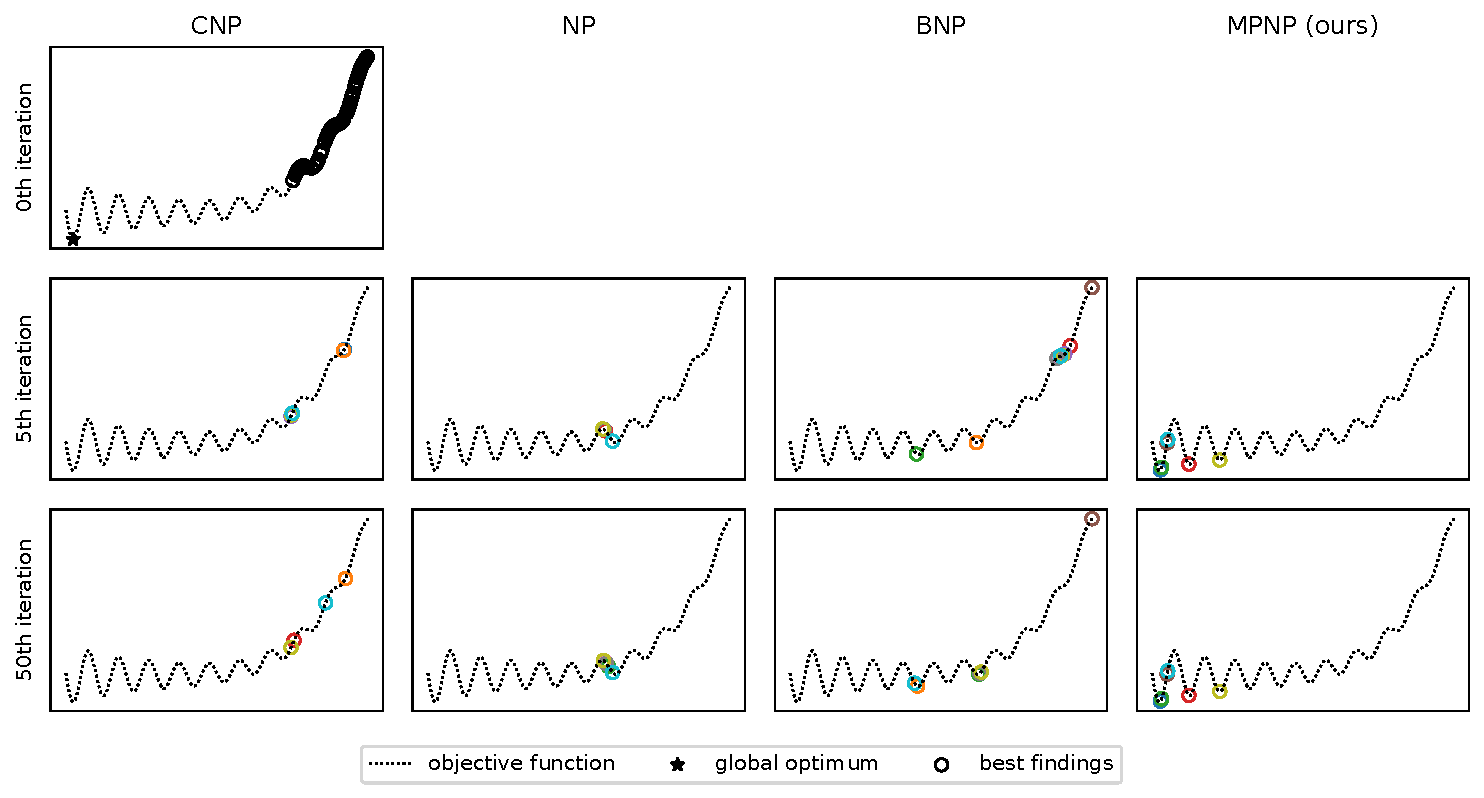
\includegraphics[width=\linewidth]{figure/app_visualize_bo_gram_np.pdf}
\caption{\citet{gramacy2012cases} function}
\end{subfigure}
\bigskip

\begin{subfigure}[b]{\textwidth}
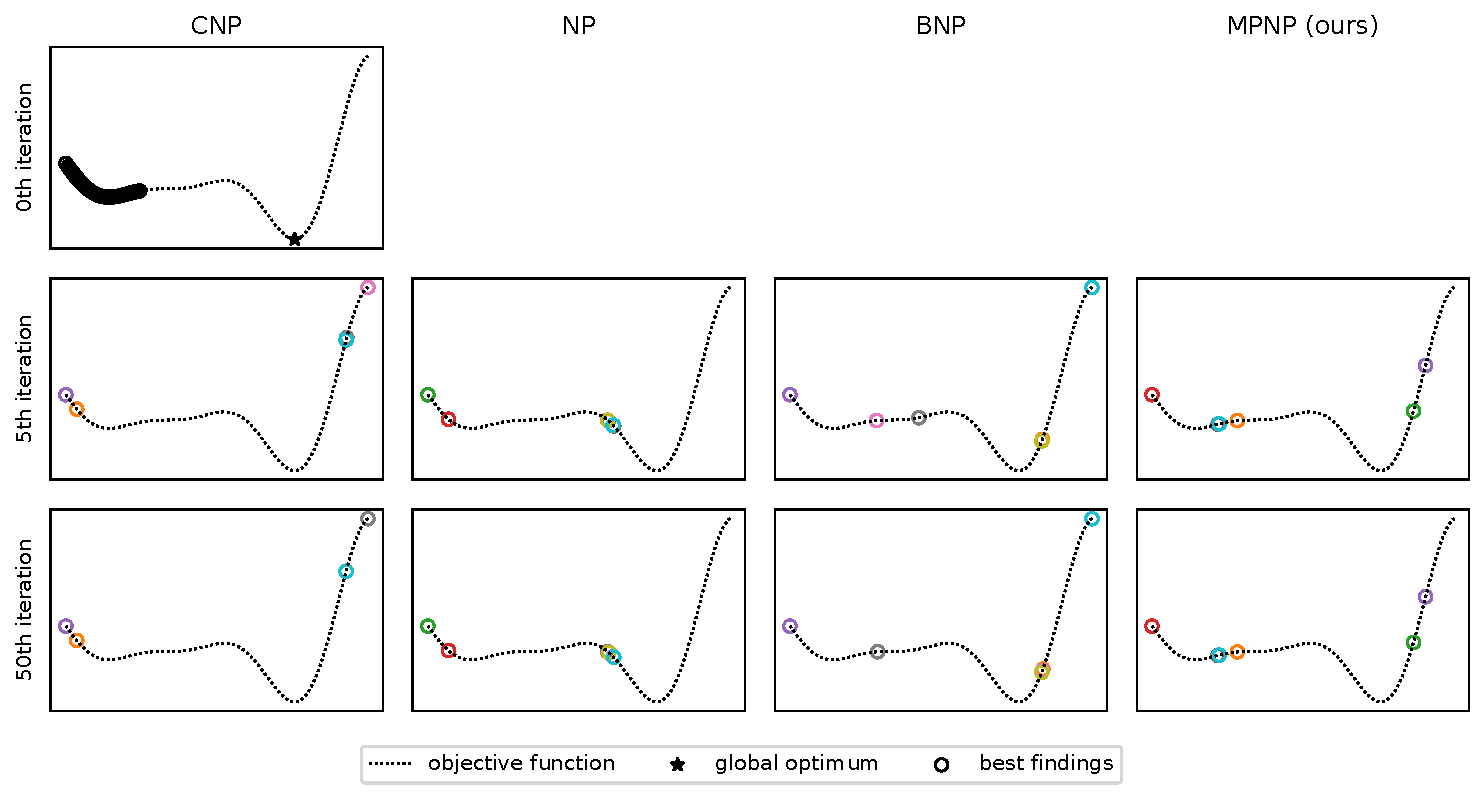
\includegraphics[width=\linewidth]{figure/app_visualize_bo_sob_np.pdf}
\caption{\citet{sobester2008engineering} function}
\end{subfigure}
\caption{It depicts 10 solutions predicted by \gls{cnp}, \gls{np}, \gls{bnp}, and \gls{mpnp}. (a,b) Predicted results for \citet{gramacy2012cases} function and \citet{sobester2008engineering} function, respectively. (Row 1) Black circles indicate the whole initial points. (Row 2) It shows the 10 best solutions predicted by each models after the 5 iterations. (Row 3) It shows the 10 best solutions predicted by each models after the whole iterations.}
\label{figure/app_visualize_bo_np}
\end{figure}

\begin{figure}
\centering
\begin{subfigure}[b]{\textwidth}
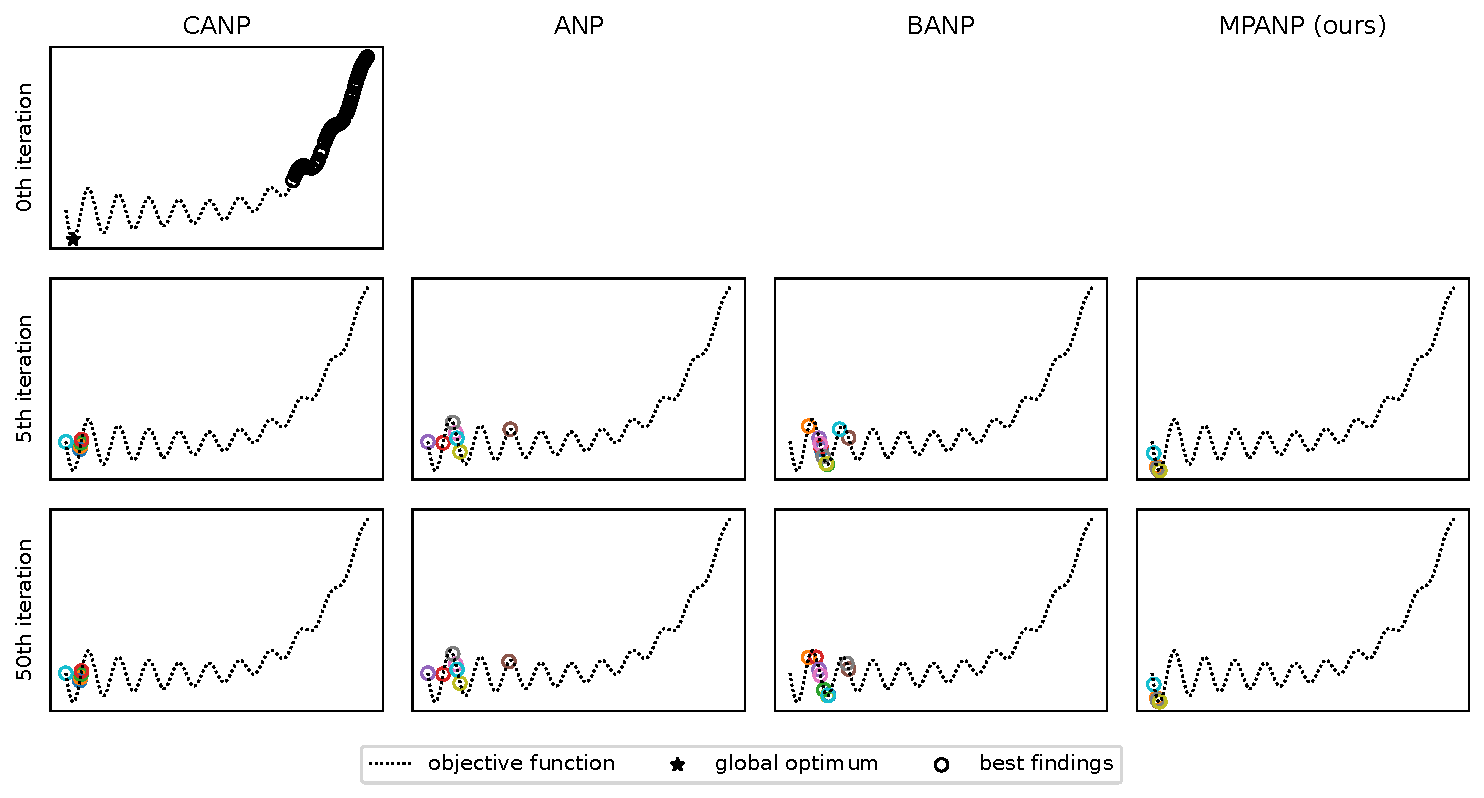
\includegraphics[width=\linewidth]{figure/app_visualize_bo_gram_anp.pdf}
\caption{\citet{gramacy2012cases} function}
\end{subfigure}
\bigskip

\begin{subfigure}[b]{\textwidth}
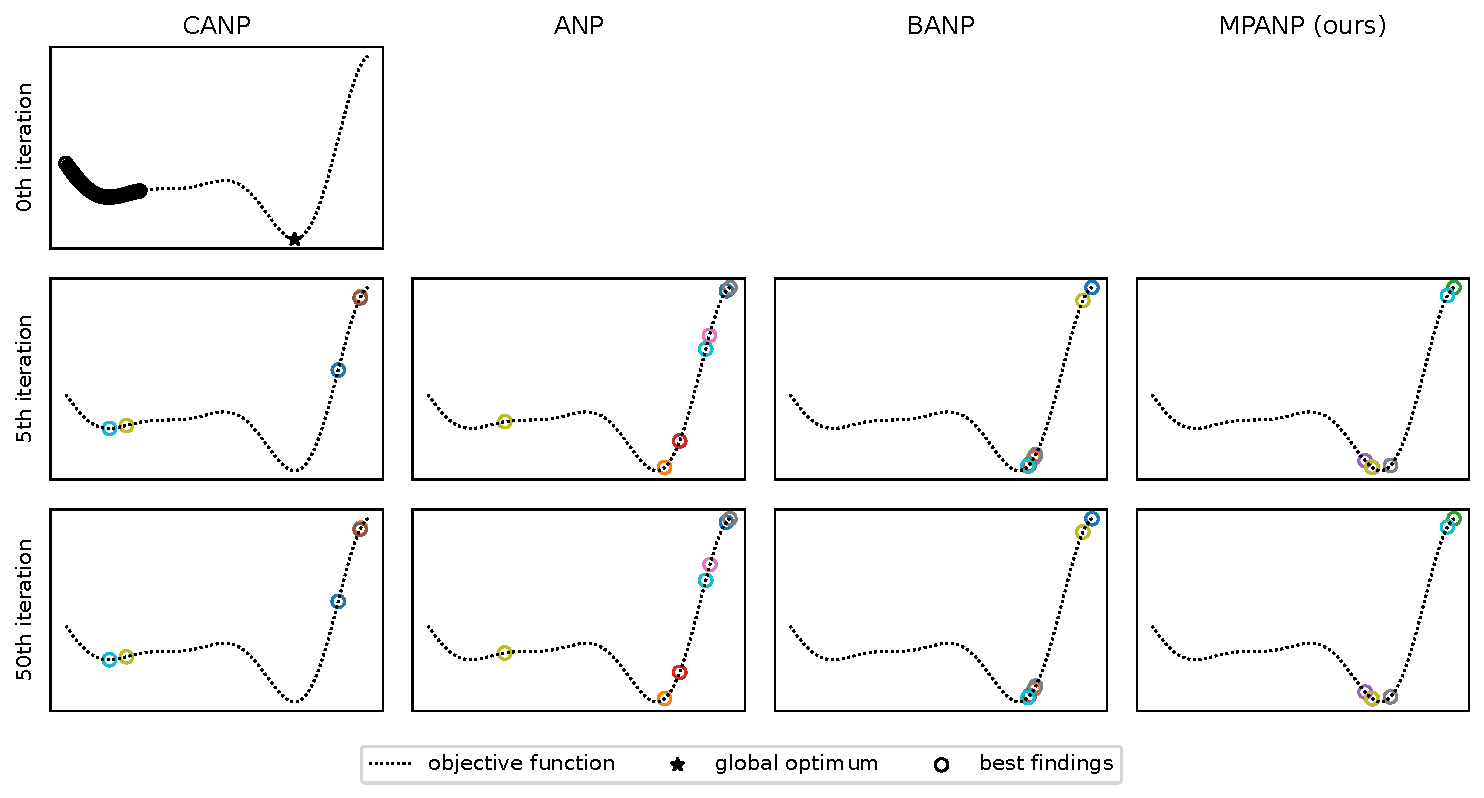
\includegraphics[width=\linewidth]{figure/app_visualize_bo_sob_anp.pdf}
\caption{\citet{sobester2008engineering} function}
\end{subfigure}
\caption{It depicts 10 solutions predicted by \gls{canp}, \gls{anp}, \gls{banp}, and \gls{mpanp}. (a,b) Predicted results for \citet{gramacy2012cases} function and \citet{sobester2008engineering} function, respectively. (Row 1) Black circles indicate the whole initial points. (Row 2) It shows the 10 best solutions predicted by each models after the 5 iterations. (Row 3) It shows the 10 best solutions predicted by each models after the whole iterations.}
\label{figure/app_visualize_bo_anp}
\end{figure}




% Here as the generator increases the size of the encoder in \glspl{mpnp}, we also increase the size of the encoder of the baselines for the fare comparisons. 
% As you can see in \cref{tab:table_gp_inf_eq}, our model still significantly outperforms the baselines.

% \begin{table}[t]
%     \caption{Context and target log likelihood values on data sampled from Gaussian Processes with various kernel. Here we used almost the same number of parameters for models. Performances are measured over 4 seeds.\\}
%     \label{tab:table_gp_inf_eq}
%     \centering
%     \scriptsize
%     \renewcommand{\arraystretch}{0.9}
%     \resizebox{0.95\textwidth}{!}{
%     \begin{tabular}{lrrrrrrrrrrrr}
%         \toprule
%         \multirow{3}{*}{Model} & \multicolumn{2}{r}{RBF}                                   & \multicolumn{2}{r}{Matern}                                & \multicolumn{2}{r}{Periodic}                                & \multicolumn{2}{r}{$t$-noise}                               \\
%                                  \cmidrule(lr){2-3}                                          \cmidrule(lr){4-5}                                          \cmidrule(lr){6-7}                                            \cmidrule(lr){8-9}
%                               & context                     & target                      & context                     & target                      & context                      & target                       & context                      & target                       \\
%         \midrule
% CNP                    &         0.983  $\pm{0.006}$ &         0.298  $\pm{0.006}$ &         0.889  $\pm{0.010}$ &         0.140  $\pm{0.003}$ &         -0.091  $\pm{0.010}$ &         -0.742  $\pm{0.039}$ &         -0.032  $\pm{0.021}$ &         -0.724  $\pm{0.018}$ \\
% NP                     &         0.984  $\pm{0.010}$ &         0.308  $\pm{0.008}$ &         0.876  $\pm{0.004}$ &         0.148  $\pm{0.006}$ &         -0.325  $\pm{0.049}$ &         -0.698  $\pm{0.035}$ &         -0.016  $\pm{0.022}$ &         -0.677  $\pm{0.039}$ \\
% BNP                    &         1.042  $\pm{0.007}$ &         0.371  $\pm{0.003}$ &         0.904  $\pm{0.013}$ &         0.176  $\pm{0.006}$ &         -0.087  $\pm{0.004}$ &         -0.738  $\pm{0.022}$ &         -0.042  $\pm{0.051}$ &         -0.664  $\pm{0.021}$ \\
% % NeuBNP                 &         0.954  $\pm{0.010}$ &         0.284  $\pm{0.004}$ &         0.861  $\pm{0.014}$ &         0.130  $\pm{0.003}$ &         -0.176  $\pm{0.028}$ &         -0.797  $\pm{0.015}$ &         -0.066  $\pm{0.013}$ &         -0.683  $\pm{0.096}$ \\
% MPNP (ours)            & \textBF{1.086} $\pm{0.005}$ & \textBF{0.457} $\pm{0.002}$ & \textBF{1.005} $\pm{0.014}$ & \textBF{0.278} $\pm{0.006}$ & \textBF{-0.017} $\pm{0.013}$ & \textBF{-0.681} $\pm{0.009}$ & \textBF{ 0.119} $\pm{0.025}$ & \textBF{-0.381} $\pm{0.013}$ \\
% \cmidrule(lr){1-1}       \cmidrule(lr){2-3}                                          \cmidrule(lr){4-5}                                          \cmidrule(lr){6-7}                                            \cmidrule(lr){8-9}
% CANP                   &         1.372  $\pm{0.001}$ &         0.625  $\pm{0.005}$ &         1.370  $\pm{0.002}$ &         0.429  $\pm{0.016}$ &          1.157  $\pm{0.051}$ &         -0.748  $\pm{0.037}$ &          0.309  $\pm{0.065}$ &         -0.804  $\pm{0.049}$ \\
% ANP                    &         1.374  $\pm{0.001}$ &         0.648  $\pm{0.016}$ &         1.371  $\pm{0.002}$ &         0.462  $\pm{0.020}$ &          1.191  $\pm{0.054}$ &         -0.709  $\pm{0.024}$ &          0.695  $\pm{0.048}$ &         -0.750  $\pm{0.082}$ \\
% BANP                   &         1.372  $\pm{0.000}$ &         0.653  $\pm{0.014}$ &         1.370  $\pm{0.002}$ &         0.450  $\pm{0.006}$ & \textBF{ 1.243} $\pm{0.083}$ &         -0.647  $\pm{0.028}$ &          0.437  $\pm{0.034}$ &         -0.645  $\pm{0.057}$ \\
% % NeuBANP                &         1.358  $\pm{0.001}$ &         0.661  $\pm{0.003}$ &         1.352  $\pm{0.001}$ &         0.477  $\pm{0.004}$ &          0.721  $\pm{0.018}$ &         -0.790  $\pm{0.007}$ &          0.763  $\pm{0.060}$ &         -0.460  $\pm{0.019}$ \\
% MPANP (ours)           & \textBF{1.374} $\pm{0.000}$ & \textBF{0.698} $\pm{0.007}$ & \textBF{1.373} $\pm{0.001}$ & \textBF{0.501} $\pm{0.005}$ &          1.167  $\pm{0.047}$ & \textBF{-0.628} $\pm{0.027}$ & \textBF{ 0.773} $\pm{0.039}$ & \textBF{-0.446} $\pm{0.057}$ \\
% % CNP                    &         0.964  $\pm{0.006}$ &         0.288  $\pm{0.006}$ &         0.859  $\pm{0.009}$ &         0.124  $\pm{0.011}$ &         -0.139  $\pm{0.007}$ &         -0.742  $\pm{0.011}$ &         -0.012  $\pm{0.021}$ &         -0.760  $\pm{0.025}$ \\
% % NP                     &         0.953  $\pm{0.003}$ &         0.306  $\pm{0.004}$ &         0.842  $\pm{0.015}$ &         0.133  $\pm{0.008}$ &         -0.346  $\pm{0.026}$ &         -0.698  $\pm{0.007}$ &         -0.018  $\pm{0.022}$ &         -0.656  $\pm{0.028}$ \\
% % BNP                    &         1.020  $\pm{0.006}$ &         0.372  $\pm{0.006}$ &         0.929  $\pm{0.008}$ &         0.206  $\pm{0.006}$ &         -0.036  $\pm{0.031}$ &         -0.738  $\pm{0.011}$ &         -0.051  $\pm{0.051}$ &         -0.670  $\pm{0.023}$ \\
% % NeuBNP                 &         0.929  $\pm{0.011}$ &         0.275  $\pm{0.007}$ &         0.834  $\pm{0.008}$ &         0.122  $\pm{0.004}$ &         -0.231  $\pm{0.010}$ &         -0.785  $\pm{0.023}$ &          0.038  $\pm{0.009}$ &         -0.516  $\pm{0.018}$ \\
% % MPNP (ours)            & \textBF{1.086} $\pm{0.005}$ & \textBF{0.457} $\pm{0.002}$ & \textBF{1.005} $\pm{0.014}$ & \textBF{0.278} $\pm{0.006}$ & \textBF{-0.017} $\pm{0.013}$ & \textBF{-0.681} $\pm{0.009}$ & \textBF{ 0.119} $\pm{0.025}$ & \textBF{-0.381} $\pm{0.013}$ \\
% % \cmidrule(lr){1-1}       \cmidrule(lr){2-3}                                          \cmidrule(lr){4-5}                                          \cmidrule(lr){6-7}                                            \cmidrule(lr){8-9}
% % CANP                   &         1.372  $\pm{0.000}$ &         0.611  $\pm{0.008}$ &         1.370  $\pm{0.001}$ &         0.423  $\pm{0.004}$ &          1.168  $\pm{0.051}$ &         -0.747  $\pm{0.037}$ &          0.404  $\pm{0.057}$ &         -1.036  $\pm{0.103}$ \\
% % ANP                    &         1.372  $\pm{0.003}$ &         0.617  $\pm{0.027}$ &         1.372  $\pm{0.001}$ &         0.432  $\pm{0.025}$ & \textBF{1.178}  $\pm{0.054}$ &         -0.719  $\pm{0.024}$ &          0.708  $\pm{0.054}$ &         -0.728  $\pm{0.093}$ \\
% % BANP                   & \textBF{1.374} $\pm{0.001}$ &         0.663  $\pm{0.002}$ &         1.371  $\pm{0.002}$ &         0.472  $\pm{0.003}$ &          0.754  $\pm{0.083}$ &         -0.913  $\pm{0.028}$ &          0.477  $\pm{0.008}$ &         -0.660  $\pm{0.059}$ \\
% % NeuBANP                &         1.357  $\pm{0.002}$ &         0.651  $\pm{0.005}$ &         1.352  $\pm{0.002}$ &         0.473  $\pm{0.007}$ &          0.697  $\pm{0.022}$ &         -0.779  $\pm{0.013}$ &          0.670  $\pm{0.028}$ &         -0.450  $\pm{0.014}$ \\
% % MPANP (ours)           & \textBF{1.374} $\pm{0.000}$ & \textBF{0.698} $\pm{0.007}$ & \textBF{1.373} $\pm{0.001}$ & \textBF{0.501} $\pm{0.005}$ &         1.167 $\pm{0.047}$ & \textBF{-0.628} $\pm{0.027}$ & \textBF{ 0.773} $\pm{0.039}$ & \textBF{-0.446} $\pm{0.057}$ \\
%         \bottomrule
%     \end{tabular}}
% \end{table}
% In this section, we report the experiment results with the baselines with increased number of parameters to match the additional number of parameters introduced for the generator in \glspl{mpnp}.
% Here as the generator increases the size of the encoder in \glspl{mpnp}, we also increase the size of the encoder of the baselines for the fare comparisons. 
% As you can see in \cref{tab:table_gp_inf_eq}, our model still significantly outperforms the baselines.

% \subsection{Finite Training Dataset Other Kernels}
% \begin{figure}[t]
%     \centering
%     % 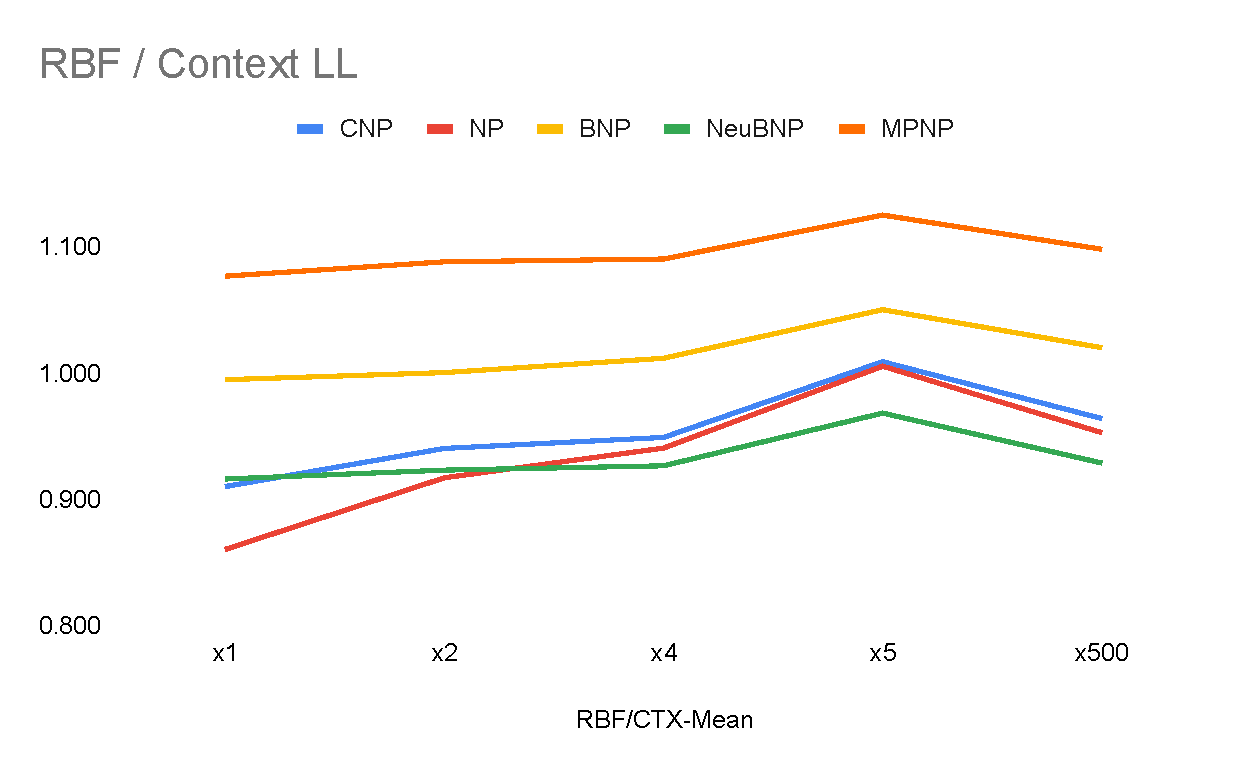
\includegraphics[width=0.24\textwidth]{figure/gp_finite/rbf_ctx_cnps.pdf}
%     % 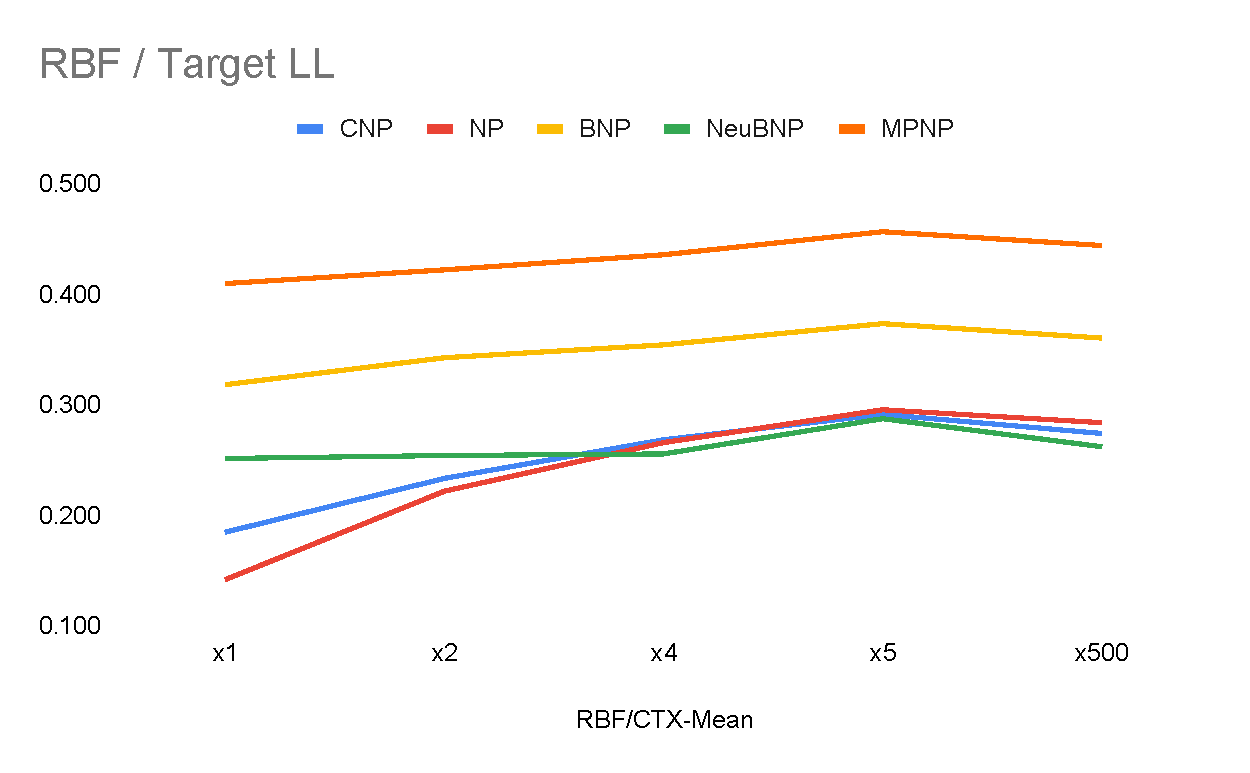
\includegraphics[width=0.24\textwidth]{figure/gp_finite/rbf_tar_cnps.pdf}
%     % 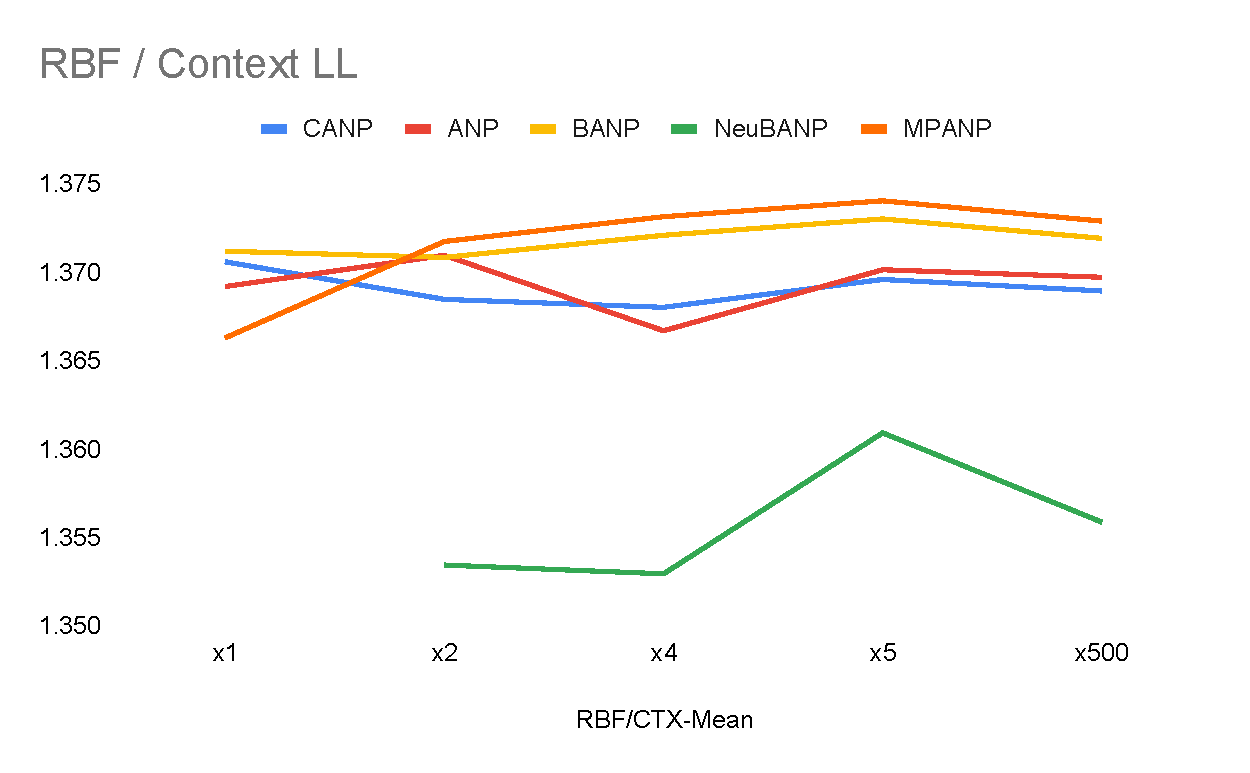
\includegraphics[width=0.24\textwidth]{figure/gp_finite/rbf_ctx_canps.pdf}
%     % 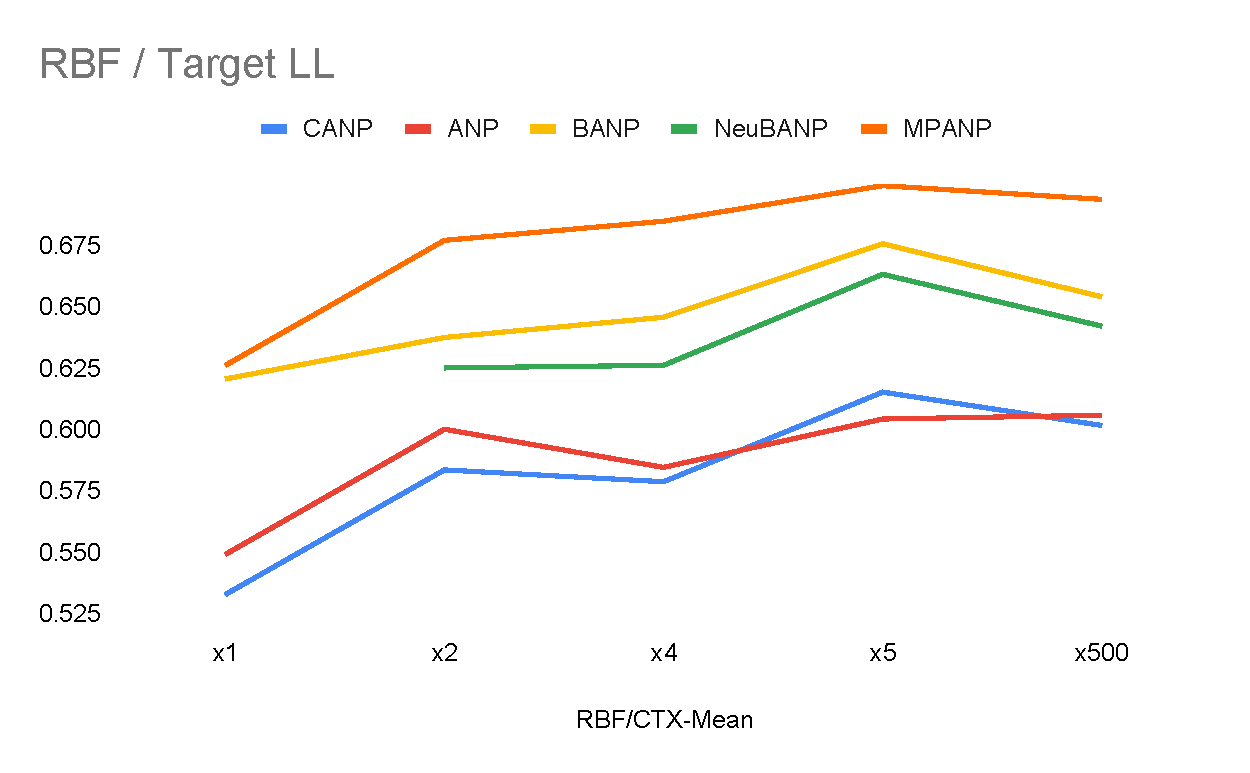
\includegraphics[width=0.24\textwidth]{figure/gp_finite/rbf_tar_canps.pdf}
%     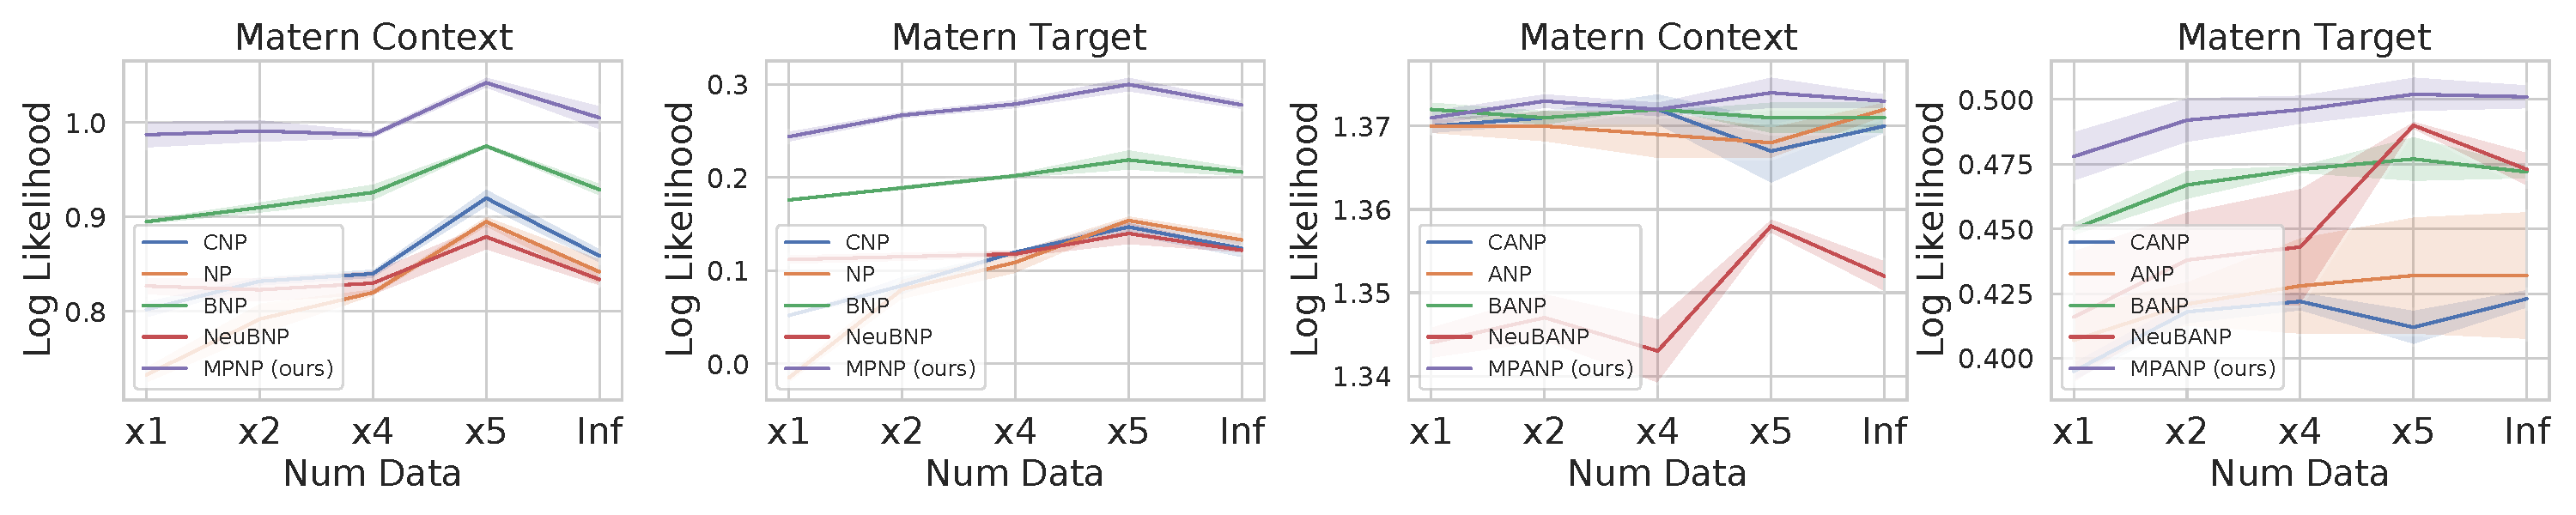
\includegraphics[width=\textwidth]{figure/out_matern.pdf}
%     \caption{Results of Finite Training Dataset experiments with Matern 5/2 kernel.}
%     \label{fig:figure_gp_finite_matern}
% \end{figure}
% \begin{figure}[t]
%     \centering
%     % 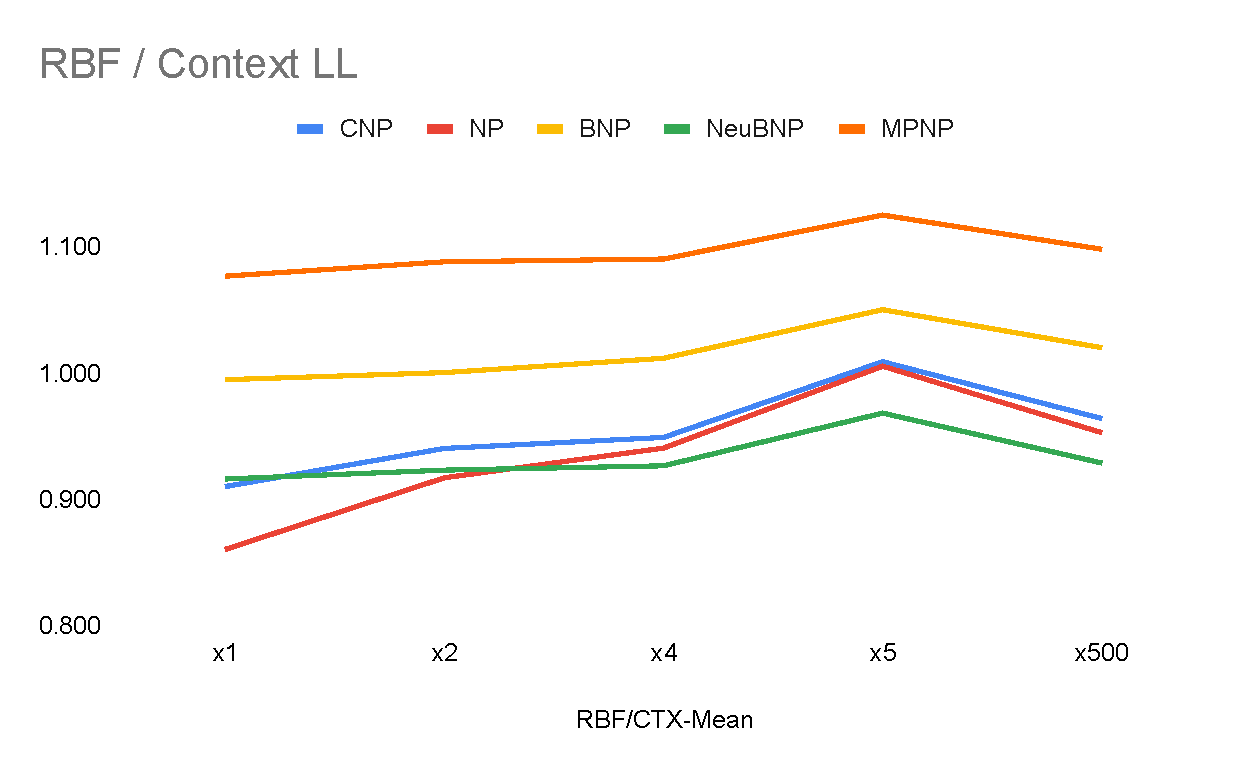
\includegraphics[width=0.24\textwidth]{figure/gp_finite/rbf_ctx_cnps.pdf}
%     % 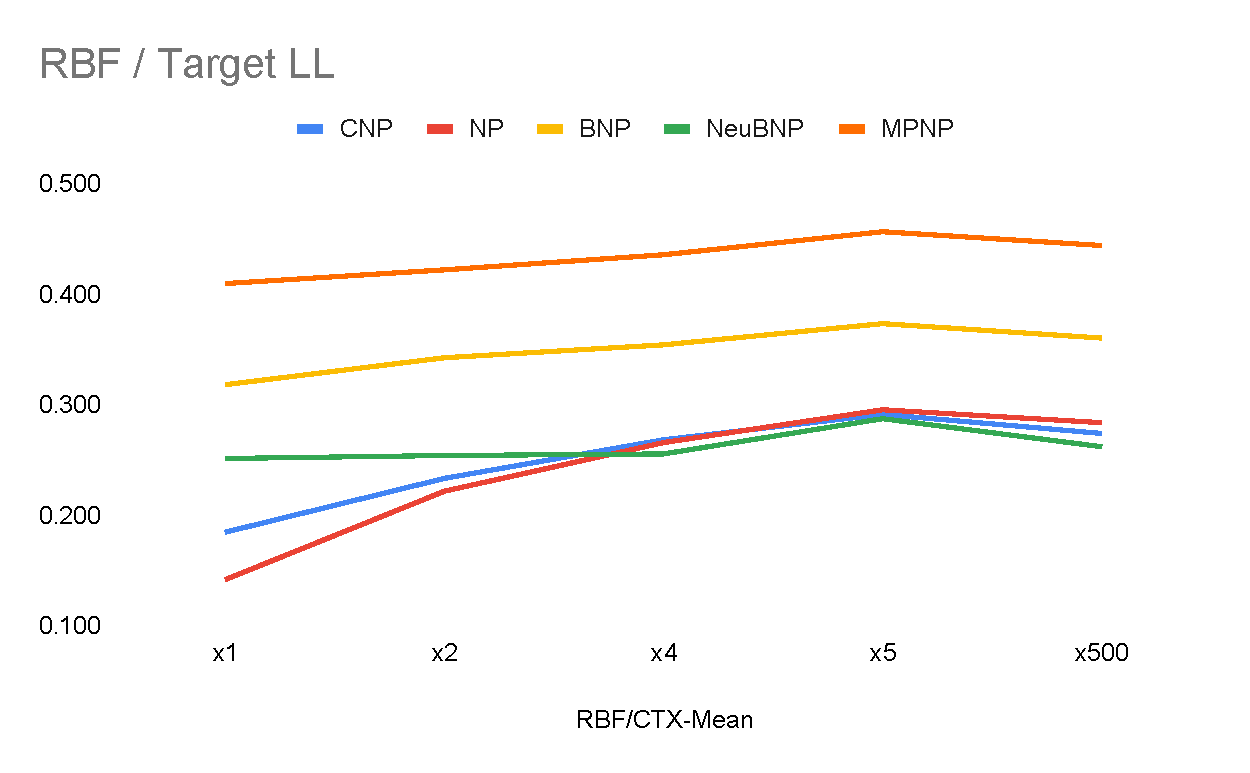
\includegraphics[width=0.24\textwidth]{figure/gp_finite/rbf_tar_cnps.pdf}
%     % 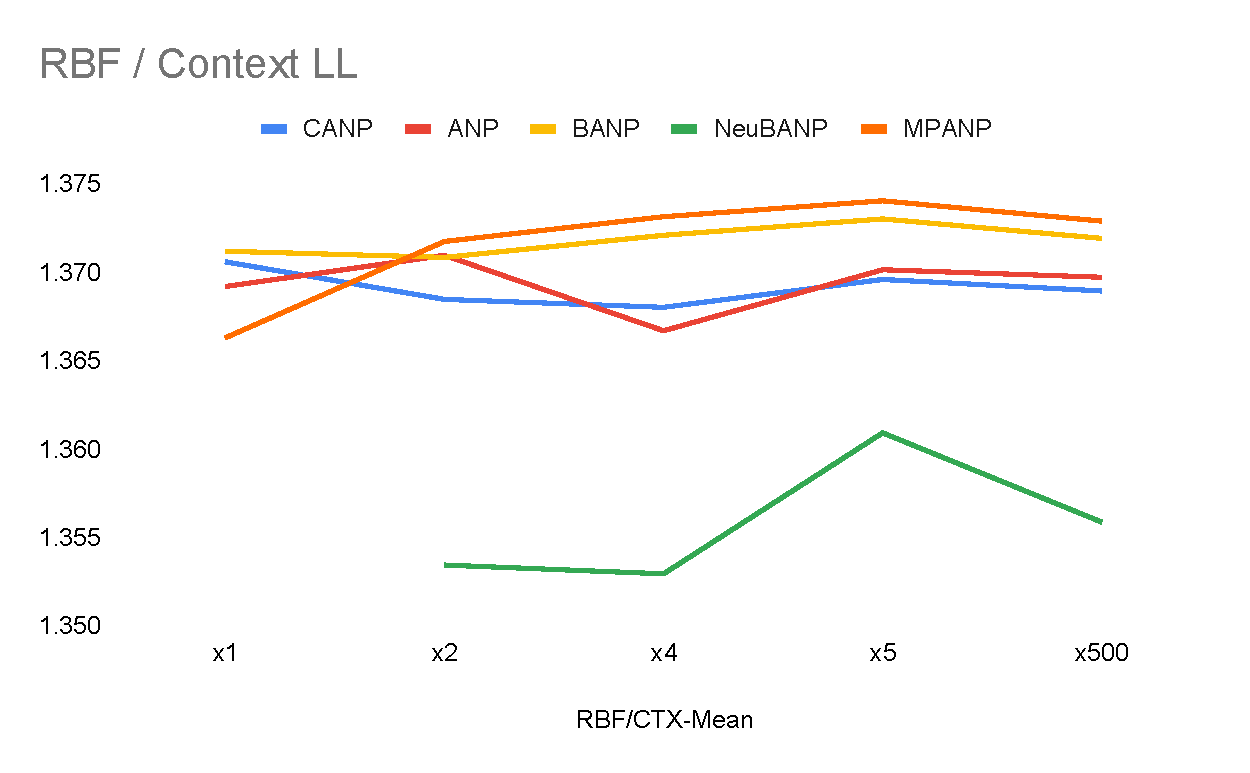
\includegraphics[width=0.24\textwidth]{figure/gp_finite/rbf_ctx_canps.pdf}
%     % 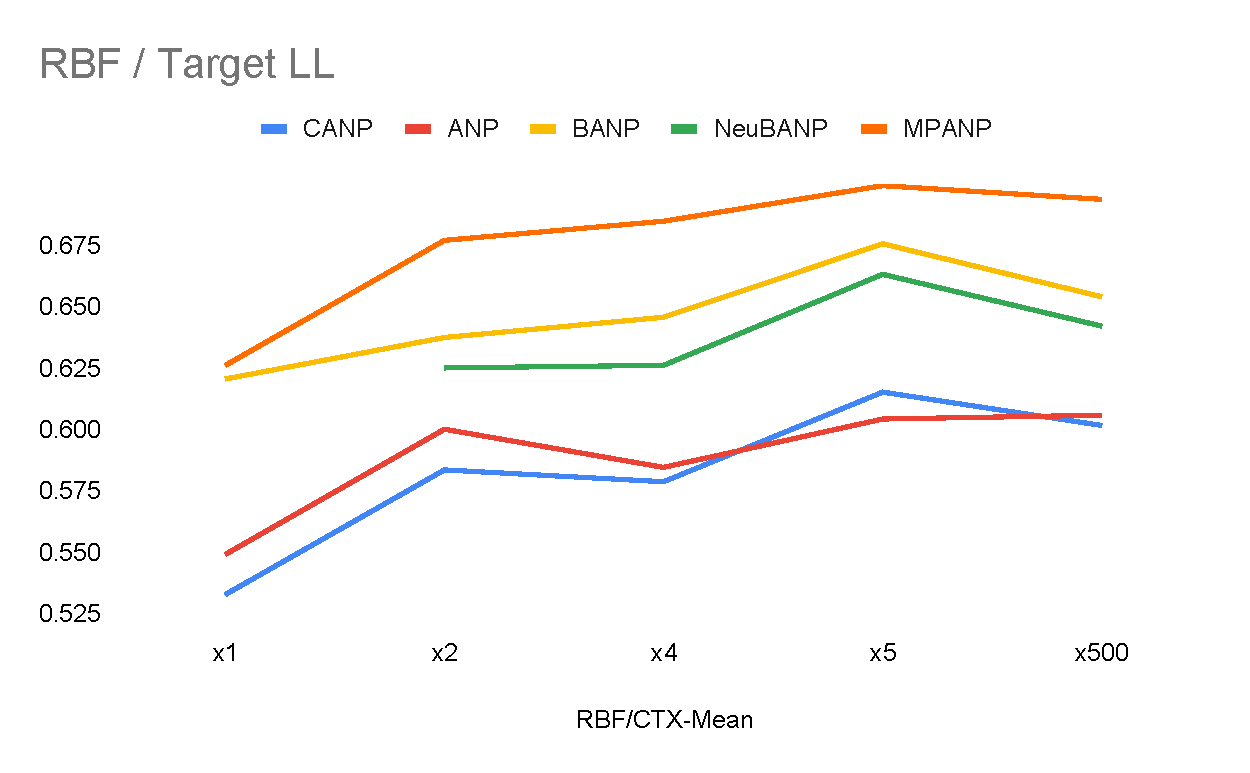
\includegraphics[width=0.24\textwidth]{figure/gp_finite/rbf_tar_canps.pdf}
%     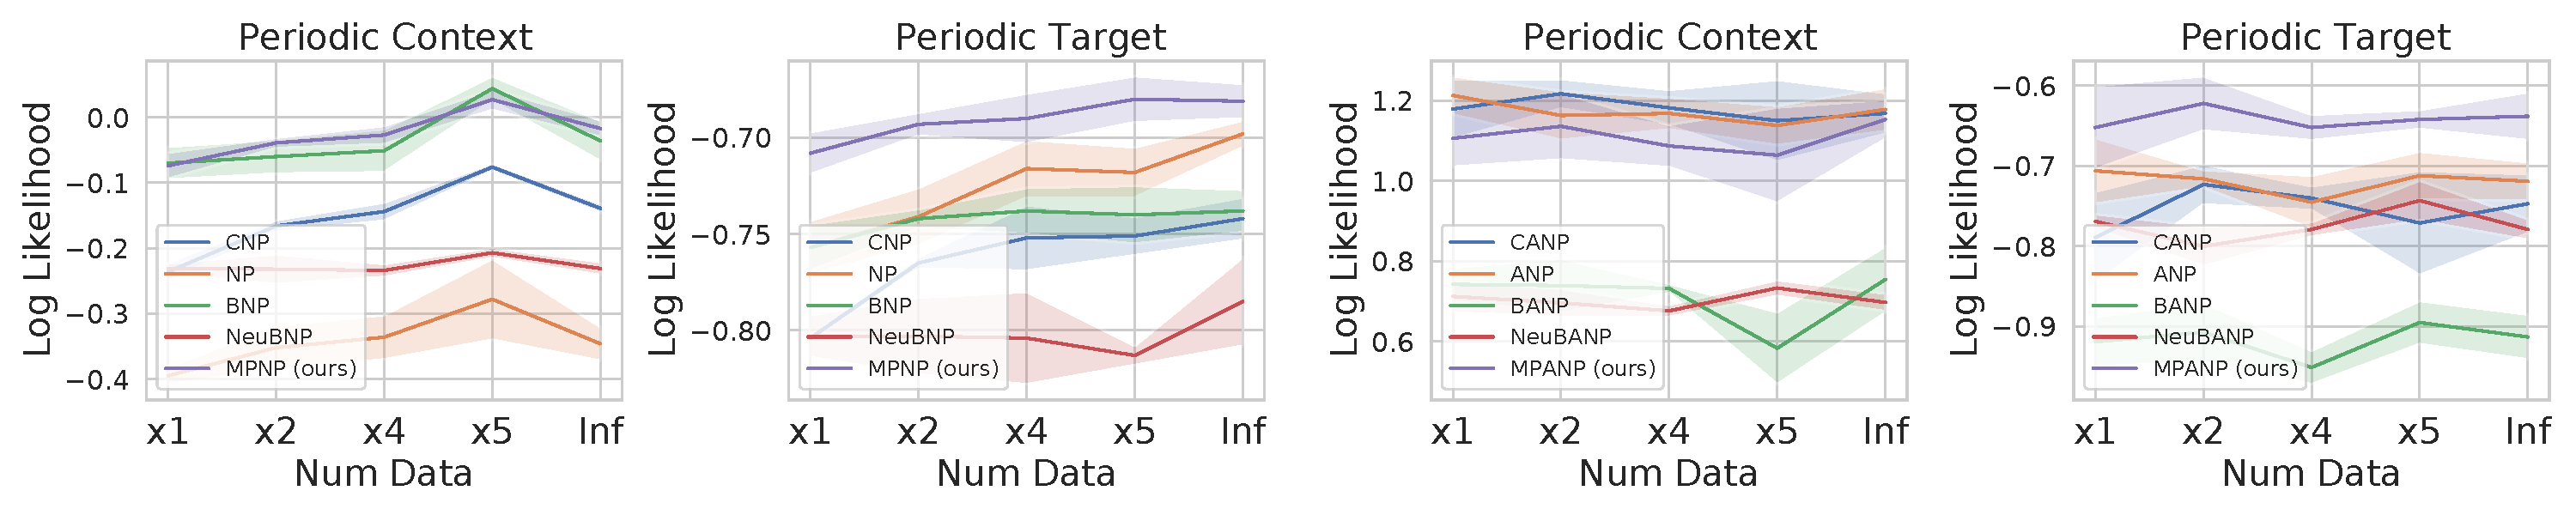
\includegraphics[width=\textwidth]{figure/out_periodic.pdf}
%     \caption{Results of Finite Training Dataset experiments with Periodic kernel.}
%     \label{fig:figure_gp_finite_periodic}
% \end{figure}
% \begin{figure}[t]
%     \centering
%     % 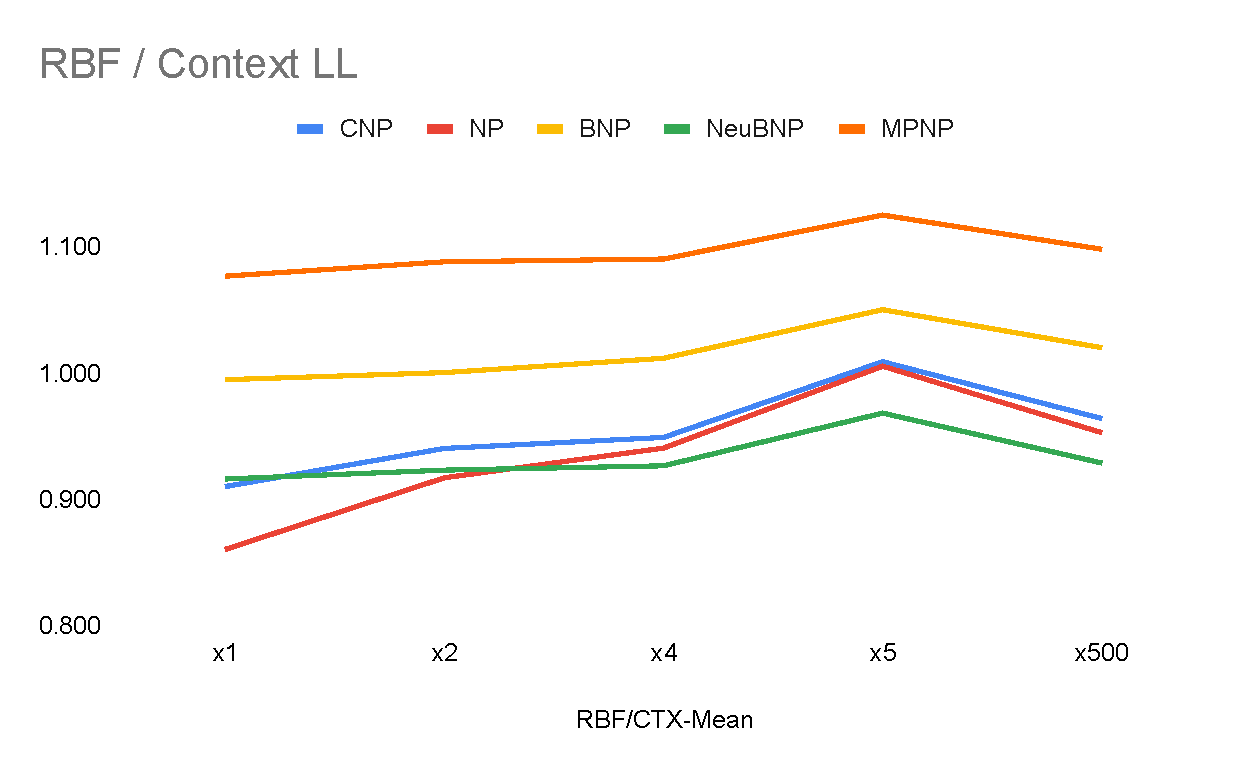
\includegraphics[width=0.24\textwidth]{figure/gp_finite/rbf_ctx_cnps.pdf}
%     % 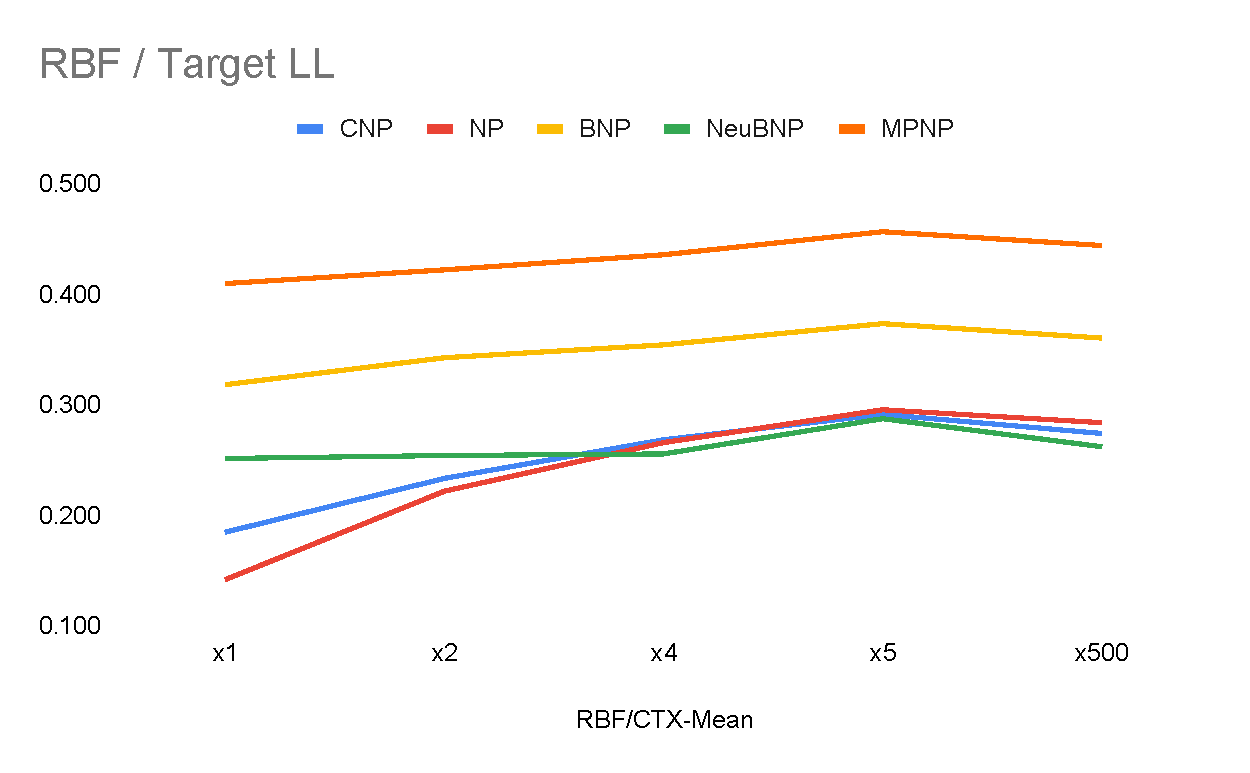
\includegraphics[width=0.24\textwidth]{figure/gp_finite/rbf_tar_cnps.pdf}
%     % 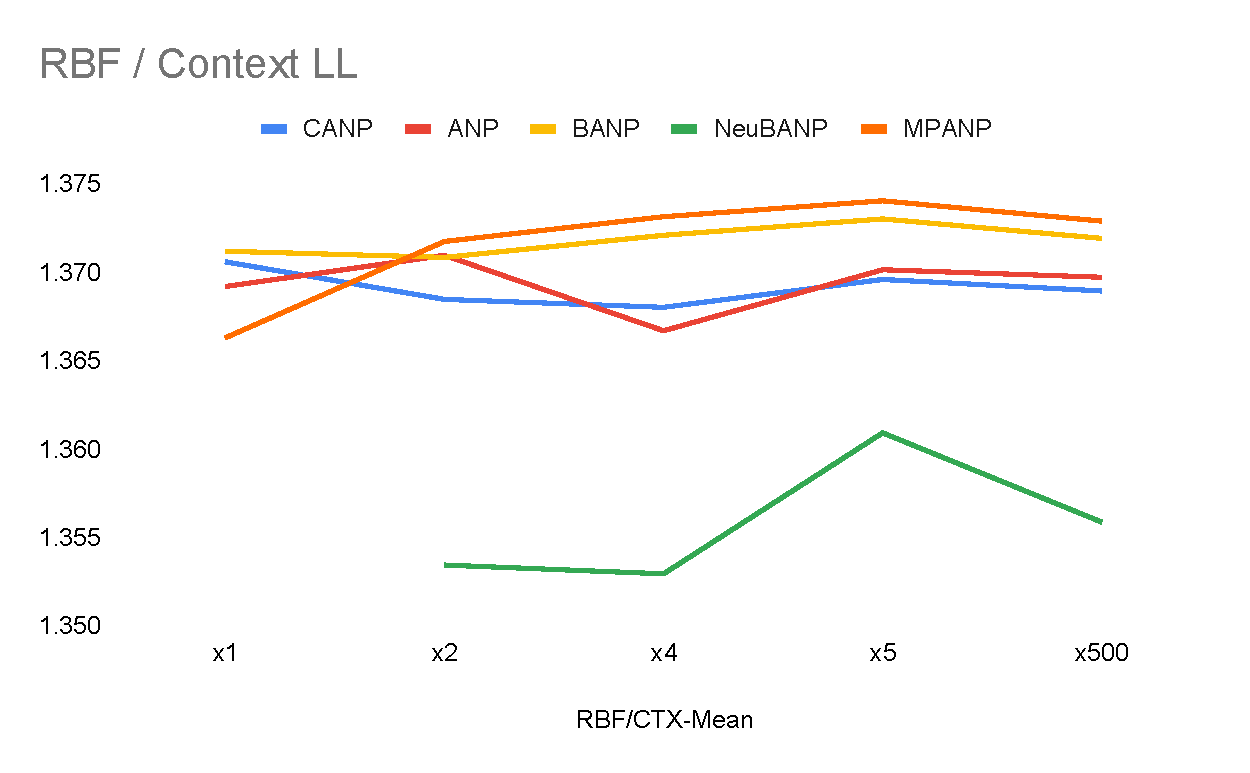
\includegraphics[width=0.24\textwidth]{figure/gp_finite/rbf_ctx_canps.pdf}
%     % 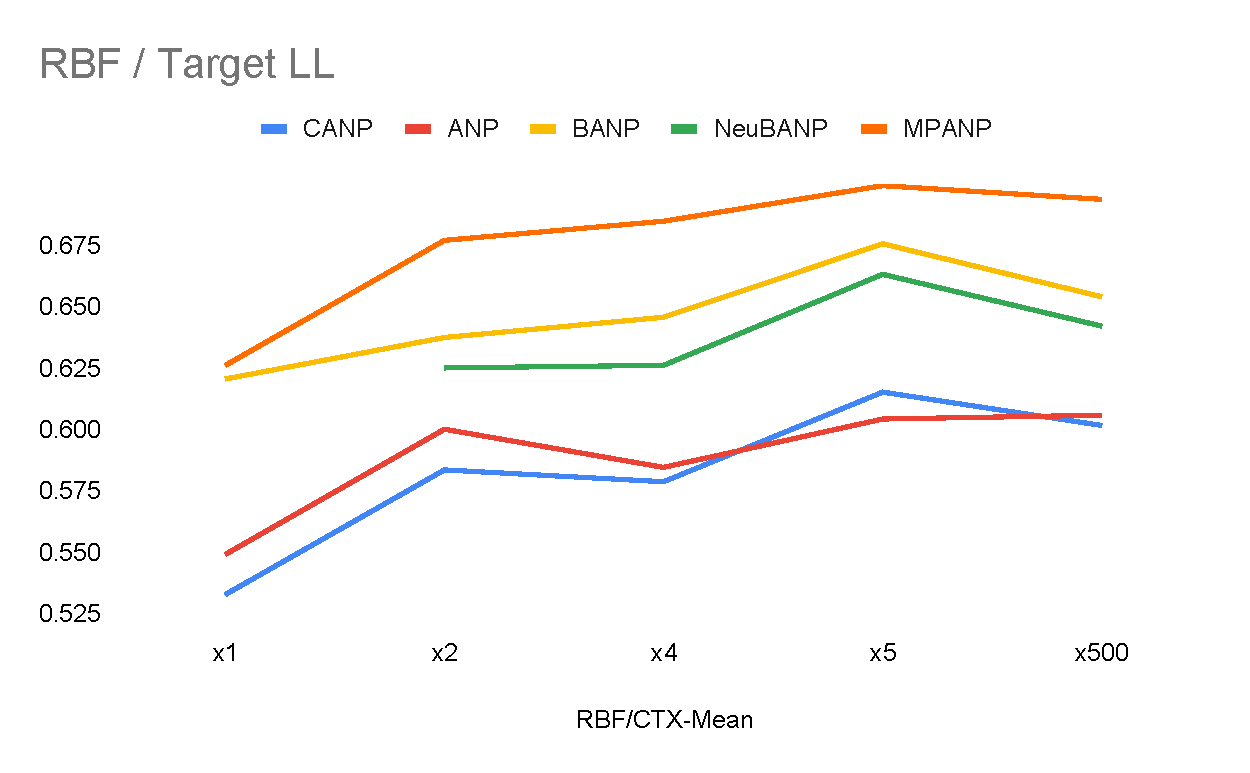
\includegraphics[width=0.24\textwidth]{figure/gp_finite/rbf_tar_canps.pdf}
%     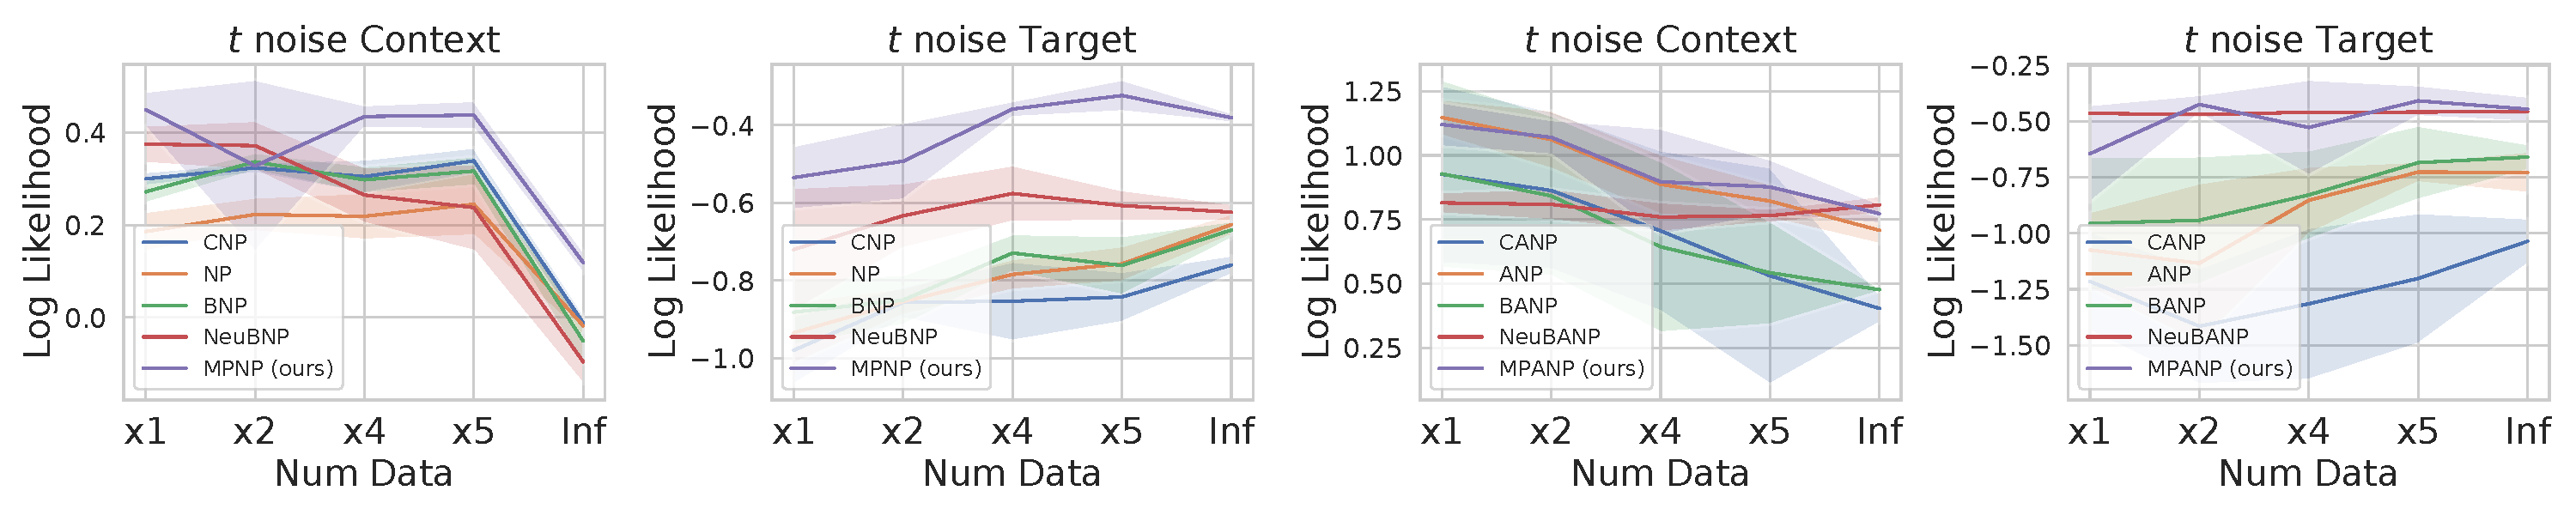
\includegraphics[width=\textwidth]{figure/out_t_noise.pdf}
%     \caption{Results of Finite Training Dataset experiments with RBF kernel with Students' $t$ distributed noise.}
%     \label{fig:figure_gp_finite_t_noise}
% \end{figure}
% In this section, we presents the remain results of Finite Training Dataset in \cref{main:subsec:infinite_training} for the kernels other than RBF.
% Here as you can see in \cref{fig:figure_gp_finite_matern}, \cref{fig:figure_gp_finite_periodic} and \cref{fig:figure_gp_finite_t_noise}, \glspl{mpnp} consistently outperforms the baselines.

% \subsection{Predator-Prey Model}
% \label{app:subsec:predator-prey}
% \begin{table}[t]
    \caption{Context and target log likelihood values on Lotka Volterra simulated data and real data. Performances are measured over 4 seeds.\\}
    \label{tab:table_lotka}
    \centering
    \scriptsize
    \renewcommand{\arraystretch}{0.9}
    \resizebox{0.6\textwidth}{!}{
    \begin{tabular}{lrrrr}
        \toprule
        \multirow{3}{*}{Model} & \multicolumn{2}{r}{Simulation}                            & \multicolumn{2}{r}{Real}                                    \\
                                 \cmidrule(lr){2-3}                                          \cmidrule(lr){4-5}                                       
                               & context                     & target                      & context                     & target                        \\
        \midrule
        CNP                    &         0.161  $\pm{0.038}$ &        -0.192  $\pm{0.032}$ &         -2.759  $\pm{0.027}$ &         -3.278  $\pm{0.041}$ \\
        NP                     &         0.185  $\pm{0.036}$ &        -0.152  $\pm{0.037}$ &         -2.707  $\pm{0.027}$ &         -3.200  $\pm{0.042}$ \\
        BNP                    &         0.402  $\pm{0.009}$ &         0.038  $\pm{0.018}$ &         -2.723  $\pm{0.032}$ &         -3.168  $\pm{0.041}$ \\
        NeuBNP                 &         0.114  $\pm{0.059}$ &        -0.267  $\pm{0.053}$ &         -2.794  $\pm{0.073}$ &         -3.128  $\pm{0.045}$ \\
        MPNP (ours)            & \textBF{0.403} $\pm{0.047}$ & \textBF{0.116} $\pm{0.035}$ & \textBF{-2.648} $\pm{0.041}$ & \textBF{-3.106} $\pm{0.021}$ \\
        \cmidrule(lr){1-1}       \cmidrule(lr){2-3}                                          \cmidrule(lr){4-5}                                       
        CANP                   &         2.498  $\pm{0.018}$ &         1.541  $\pm{0.010}$ &          1.836  $\pm{0.169}$ &         -6.873  $\pm{0.612}$ \\
        ANP                    &         2.528  $\pm{0.026}$ &         1.643  $\pm{0.011}$ & \textBF{ 2.058} $\pm{0.080}$ &         -5.454  $\pm{0.408}$ \\
        BANP                   & \textBF{2.605} $\pm{0.021}$ &         1.685  $\pm{0.032}$ &          2.054  $\pm{0.126}$ & \textBF{-3.388} $\pm{0.446}$ \\
        NeuBANP                &         2.421  $\pm{0.024}$ &         1.358  $\pm{0.026}$ &          1.878  $\pm{0.050}$ &         -3.739  $\pm{0.240}$ \\
        MPANP (ours)           &         2.554  $\pm{0.025}$ & \textBF{1.769} $\pm{0.013}$ &          1.946  $\pm{0.136}$ &         -4.942  $\pm{0.387}$ \\
        \bottomrule
    \end{tabular}}
\end{table}
% Following \citet{lee2020bootstrapping}, we conducted the predator-prey population regression experiments.
% We first trained the models using the simulation datasets which are generated from a Lotka-Volterra model~\citep{wilkinson2018stochastic} with the simulation settings followed by \citet{lee2020bootstrapping}. Then tested on the generated simulation test dataset and real-world dataset which is called Hudson's Bay hare-lynx data.
% As mentioned in \citet{lee2020bootstrapping}, the real-world dataset shows different tendency from generated simulation datasets, so we can also treat this experiment as model-data mismatch experiments.
% In \cref{tab:table_lotka}, we can see that \glspl{mpnp} outperforms the other baselines for the test simulation datasets but underperforms in the real-world dataset compare to other baselines especially in the \gls{mpanp} case.
% This also shows that model-data mismatch is an open problem for the \glspl{mpnp}. 
